\documentclass[aspectratio=1610, 9pt]{beamer}
\usepackage{mobi-beamer}

\title[Simulación Monte Carlo: estimación,…]{Simulación Monte Carlo: estimación, error y distribución de salida}
\subtitle{}
\author{Alejandra Tabares Pozos}
\institute{Universidad de los Andes \\
 Departamento de Ingeniería Industrial}
\date{}

\begin{document}

%================================================
% SLIDE 1: PORTADA
%================================================
\begin{frame}
  \titlepage
\end{frame}

%================================================
% SLIDE 2: CONTINUIDAD CON LA INTRO
%================================================
\begin{frame}{¿Dónde encaja Monte Carlo en lo que ya vimos?}
\begin{block}{Recordatorio conceptual (de la clase anterior)}
Modelamos incertidumbre con una entrada aleatoria $\xi$ y definimos un resultado de interés
\[
Y = g(\xi).
\]
En problemas reales, el ``cálculo exacto'' suele ser una integral o esperanza:
\[
\mathbb E[Y] = \int_\Omega g(\xi(\omega))\, d\mathbb P(\omega).
\]
\end{block}

\begin{alertblock}{La idea de Monte Carlo}
Reemplazar una esperanza difícil por un promedio muestral construido a partir de réplicas del experimento aleatorio.
\end{alertblock}

\medskip
En esta clase vamos a hacer explícitas tres capas: \emph{(i) qué se estima}, \emph{(ii) con qué error}, y \emph{(iii) qué nos dice la distribución de salida (no solo la media)}.
\end{frame}

%================================================
% SLIDE 3: RÉPLICA / ESCENARIO + ESTIMADOR
%================================================
\begin{frame}{Réplica (escenario) y estimador: el objeto matemático}
\begin{block}{Qué es una réplica}
Una \textbf{réplica} es una realización independiente de la entrada aleatoria $\xi$:
\[
\xi^{(1)},\xi^{(2)},\dots,\xi^{(N)} \quad \text{i.i.d.}
\]
y produce una colección de salidas:
\[
Y_i = g\!\left(\xi^{(i)}\right),\qquad i=1,\dots,N.
\]
Cada $Y_i$ es un número (una ``corrida'') pero, como $\xi^{(i)}$ es aleatoria, $Y_i$ también lo es.
\end{block}

\begin{block}{Qué es un estimador}
Si el parámetro de interés es $\mu=\mathbb E[Y]$, el estimador Monte Carlo es el promedio:
\[
\widehat\mu_N=\frac{1}{N}\sum_{i=1}^N Y_i.
\]
\end{block}

\end{frame}


\begin{frame}{Definición: simulación Monte Carlo}
\begin{block}{Definición (operativa)}
La \textbf{simulación Monte Carlo} es un método numérico que aproxima cantidades probabilísticas
(\emph{esperanzas, probabilidades, cuantiles}) mediante \textbf{muestreo repetido} del modelo aleatorio.
\end{block}

\medskip
\textbf{Marco matemático:} sea $\xi$ una entrada aleatoria y $Y=g(\xi)$ la salida (costo, tiempo, utilidad).
Queremos una cantidad como $\theta$:
\[
\theta \in \Big\{\ \mathbb E[Y],\ \mathbb P(Y>\tau),\ q_\alpha(Y)\ \Big\}.
\]

\begin{block}{Principio de Monte Carlo}
Generar réplicas i.i.d.\ $\xi^{(1)},\dots,\xi^{(N)}$ y calcular $Y_i=g(\xi^{(i)})$.
Luego reemplazar la cantidad teórica por su análogo muestral:
\[
\mathbb E[Y]\approx \widehat\mu_N=\frac{1}{N}\sum_{i=1}^N Y_i,
\qquad
\mathbb P(Y>\tau)\approx \frac{1}{N}\sum_{i=1}^N \mathbf 1\{Y_i>\tau\},
\qquad
q_\alpha(Y)\approx Y_{(\lceil \alpha N\rceil)}.
\]
\end{block}

\end{frame}


%================================================
% SLIDE 4: ALGORITMO MONTE CARLO (PASOS)
%================================================
\begin{frame}{Algoritmo Monte Carlo}
\begin{block}{Esqueleto del método}
Para estimar $\mathbb E[g(\xi)]$:
\begin{enumerate}
  \item Especificar el modelo probabilístico de $\xi$ (distribuciones y parámetros).
  \item Repetir $N$ veces: generar $\xi^{(i)}$ y calcular $Y_i=g(\xi^{(i)})$.
  \item Reportar $\widehat\mu_N$ y una medida de error (IC o error estándar).
\end{enumerate}
\end{block}

\begin{block}{Tres salidas típicas (no solo medias)}
A partir de $\{Y_i\}$, usualmente queremos:
\[
\mathbb E[Y],\qquad \mathbb P(Y>\tau),\qquad q_\alpha(Y)\ \text{(percentiles)}.
\]
La misma nube de simulaciones sirve para las tres, pero \emph{la precisión no cuesta igual}.
\end{block}
\end{frame}

%================================================
% SLIDE 5: LA DISTRIBUCIÓN DE SALIDA (lo omitido)
%================================================
\begin{frame}{La salida tiene distribución: $Y=g(\xi)$ induce $F_Y$}
\begin{block}{Punto probabilístico central}
Como $Y=g(\xi)$ es una variable aleatoria, tiene una distribución inducida:
\[
F_Y(y)=\mathbb P(Y\le y)=\mathbb P\big(g(\xi)\le y\big).
\]
.
\end{block}

\begin{block}{Qué estima Monte Carlo además de la media}
Con una muestra $\{Y_i\}$ podemos construir la \textbf{distribución empírica}:
\[
\widehat F_N(y)=\frac{1}{N}\sum_{i=1}^N \mathbf 1\{Y_i\le y\}.
\]
De ella salen naturalmente probabilidades $\widehat{\mathbb P}(Y>\tau)=1-\widehat F_N(\tau)$ y cuantiles por ordenamiento.
\end{block}

\begin{alertblock}{Mensaje}
La media resume; la distribución explica (riesgo, colas, percentiles). En Monte Carlo, \emph{la distribución de salida es parte del producto}.
\end{alertblock}
\end{frame}


%================================================
% BLOQUE DE EJEMPLO NUMÉRICO (para acompañar: réplica/estimador, definición MC,
% algoritmo, y distribución de salida / F_N)
% Ejemplo: inventario 1 día, demanda en dos escenarios.
%================================================

%------------------------------------------------
% SLIDE A: DEFINICIÓN DEL EJEMPLO (xi, g, Y)
%------------------------------------------------
\begin{frame}{Ejemplo numérico (1 día): demanda incierta \texorpdfstring{$\Rightarrow$}{->} costo por faltante}
\textbf{Decisión fija:} ordenar $Q=100$ unidades. \qquad \textbf{Costo por faltante:} $c_s=10$.

\medskip
\begin{block}{Modelo probabilístico de la entrada}
La demanda $D$ toma dos valores (dos escenarios):
\[
D=
\begin{cases}
80 & \text{con prob. } 0.7,\\
120 & \text{con prob. } 0.3.
\end{cases}
\]
Esto define la entrada aleatoria $\xi:=D$.
\end{block}

\begin{block}{Salida (función del azar): \texorpdfstring{$Y=g(\xi)$}{Y=g(xi)}}
Definimos el costo por faltante:
\[
Y=g(D)=c_s(D-Q)_+=10\max\{D-100,0\}.
\]
Así, si $D=80$ entonces $Y=0$; si $D=120$ entonces $Y=10\cdot 20=200$.
\end{block}
\end{frame}

%------------------------------------------------
% SLIDE B: RÉPLICAS CONCRETAS (tabla) + estimador mu_hat
%------------------------------------------------
\begin{frame}{Réplica (escenario) y estimador: números concretos}
\textbf{Una réplica} es un sorteo independiente de $D$ (y por tanto de $Y=g(D)$).

\medskip
\begin{block}{Diez réplicas (simulación manual)}
\small
\begin{center}
\begin{tabular}{@{}ccccccccccc@{}}
\toprule
$i$ & 1 & 2 & 3 & 4 & 5 & 6 & 7 & 8 & 9 & 10\\
\midrule
$D^{(i)}$ & 80 & 120 & 80 & 80 & 120 & 80 & 80 & 120 & 80 & 80\\
$Y_i=10(D^{(i)}-100)_+$ & 0 & 200 & 0 & 0 & 200 & 0 & 0 & 200 & 0 & 0\\
\bottomrule
\end{tabular}
\end{center}
\end{block}

\begin{block}{Estimador Monte Carlo de la media}
\[
\widehat\mu_{10}=\frac{1}{10}\sum_{i=1}^{10}Y_i=\frac{0+200+0+0+200+0+0+200+0+0}{10}=\frac{600}{10}=60.
\]
\end{block}

\begin{alertblock}{Lectura}
Con pocas réplicas el estimador puede variar, pero ya vemos el mecanismo: \emph{repetir y promediar}.
\end{alertblock}
\end{frame}

%------------------------------------------------
% SLIDE C: CONEXIÓN CON LA DEFINICIÓN DE MONTE CARLO (E, P, cuantil)
%------------------------------------------------
\begin{frame}{Definición de Monte Carlo (en el ejemplo): media, probabilidad y cuantil}
En este ejemplo, la nube $\{Y_i\}_{i=1}^{N}$ permite estimar varias cantidades:

\begin{block}{(1) Media: costo esperado}
\[
\mathbb E[Y]\approx \widehat\mu_N=\frac{1}{N}\sum_{i=1}^N Y_i.
\]
Con $N=10$: \ $\widehat\mu_{10}=60$.
\end{block}

\begin{block}{(2) Probabilidad: ``día con costo alto''}
Para un umbral $\tau=0$, por ejemplo:
\[
\mathbb P(Y>0)\approx \widehat\pi_N=\frac{1}{N}\sum_{i=1}^N \mathbf 1\{Y_i>0\}.
\]
En la tabla, hay 3 valores de 200 entre 10: \ $\widehat\pi_{10}=3/10=0.3$.
\end{block}
\end{frame}

\begin{frame}{Definición de Monte Carlo (en el ejemplo): media, probabilidad y cuantil}

\begin{block}{(3) Cuantil: percentil \texorpdfstring{$\alpha$}{alpha}}
Ordenamos $Y_{(1)}\le \cdots \le Y_{(N)}$ y definimos
\[
\widehat q_\alpha = Y_{(\lceil \alpha N\rceil)}.
\]
Con $N=10$, el cuantil 0.9 es $Y_{(\lceil 9\rceil)}=Y_{(9)}=200$.
\end{block}
\end{frame}

%------------------------------------------------
% SLIDE D: ALGORITMO MONTE CARLO (mapeado al ejemplo)
%------------------------------------------------
\begin{frame}{Algoritmo Monte Carlo (mapeado al ejemplo)}
\begin{block}{Paso 1: especificar el modelo de \texorpdfstring{$\xi$}{xi}}
Aquí $\xi=D$ con dos escenarios (80 con 0.7; 120 con 0.3).
\end{block}

\begin{block}{Paso 2: repetir (generar y evaluar)}
Para $i=1,\dots,N$:
\begin{enumerate}
  \item Generar $D^{(i)}\in\{80,120\}$ según las probabilidades dadas.
  \item Calcular $Y_i=g(D^{(i)})=10(D^{(i)}-100)_+$.
\end{enumerate}
\end{block}

\begin{block}{Paso 3: reportar estimaciones}
\[
\widehat{\mathbb E[Y]}=\widehat\mu_N,\qquad
\widehat{\mathbb P}(Y>\tau)=\widehat\pi_N,\qquad
\widehat q_\alpha=Y_{(\lceil \alpha N\rceil)}.
\]
\end{block}

\end{frame}

%------------------------------------------------
% SLIDE E: DISTRIBUCIÓN DE SALIDA + DISTRIBUCIÓN EMPÍRICA F_N (numérica)
%------------------------------------------------
\begin{frame}{La salida tiene distribución: \texorpdfstring{$F_Y$}{FY} y \texorpdfstring{$\widehat F_N$}{Fhat} en números}
\begin{block}{Distribución verdadera en este ejemplo}
Como $Y=g(D)$ toma solo dos valores:
\[
Y=
\begin{cases}
0 & \text{con prob. } 0.7,\\
200 & \text{con prob. } 0.3,
\end{cases}
\]
la cdf verdadera es
\[
F_Y(y)=\mathbb P(Y\le y)=
\begin{cases}
0, & y<0,\\
0.7, & 0\le y<200,\\
1, & y\ge 200.
\end{cases}
\]
\end{block}

\begin{block}{Distribución empírica con \texorpdfstring{$N=10$}{N=10} (de la tabla)}
\[
\widehat F_{10}(y)=\frac{1}{10}\sum_{i=1}^{10}\mathbf 1\{Y_i\le y\}.
\]
En nuestra muestra: hay 7 ceros y 3 doses-cientos. Entonces
\[
\widehat F_{10}(y)=
\begin{cases}
0, & y<0,\\
0.7, & 0\le y<200,\\
1, & y\ge 200,
\end{cases}
\]
que coincide exactamente con $F_Y$ (aquí tuvimos ``suerte''; con otra muestra podría diferir).
\end{block}
\end{frame}

%================================================
% SECCIÓN REEMPLAZO: LLN -> CLT -> IC (desenredada y prosaica)
% Colocar inmediatamente después del ejemplo manual (cuando ya tienen {Y_i})
%================================================

%------------------------------------------------
% SLIDE 1: DOS DISTRIBUCIONES DISTINTAS (Y vs mu_hat)
%------------------------------------------------
\begin{frame}{Dos cosas aleatorias distintas}
\begin{block}{1) La distribución del sistema (salida)}
\[
Y=g(\xi)\quad \Rightarrow \quad F_Y(y)=\mathbb P(Y\le y).
\]
Esto describe \textbf{qué tan variable es el resultado} (colas, percentiles, riesgo).
\end{block}

\begin{block}{2) La distribución del estimador (error por muestreo)}
Cuando calculamos
\[
\widehat\mu_N=\frac{1}{N}\sum_{i=1}^N Y_i,
\]
\textbf{$\widehat\mu_N$ también es aleatorio}, porque depende de la muestra.
Su distribución (si repitiéramos el experimento completo muchas veces) se llama
\emph{distribución de muestreo} de $\widehat\mu_N$.
\end{block}


Monte Carlo produce una \textbf{muestra de $Y$} (para estimar $F_Y$) y, al mismo tiempo,
produce un \textbf{estimador} (para estimar $\mu=\mathbb E[Y]$) con error.

\end{frame}

%------------------------------------------------
% SLIDE 2: LLN (qué garantiza y qué NO)
%------------------------------------------------
\begin{frame}{Ley de los Grandes Números (LLN)}
\begin{block}{LLN (consistencia del promedio)}
Si $Y_1,\dots,Y_N$ son i.i.d. y $\mathbb E[|Y|]<\infty$, entonces:
\[
\widehat\mu_N \xrightarrow[]{a.s.} \mu=\mathbb E[Y]\qquad (N\to\infty).
\]
\end{block}

\begin{block}{Qué NO te da la LLN}
LLN no te dice:
\begin{itemize}
  \item \textbf{cuánto puede estar errado} $\widehat\mu_N$ para un $N$ concreto,
  \item ni cómo construir una ``barra de error'' con cobertura 95\%.
\end{itemize}
Para eso necesitamos el \textbf{Teorema Central del Límite}.
\end{block}

\begin{alertblock}{Lectura}
LLN: ``si simulas mucho, te acercas''. \quad Pero no cuantifica el \emph{tamaño típico del error}.
\end{alertblock}
\end{frame}

%------------------------------------------------
% SLIDE 3: CLT (por qué aparece 1/sqrt(N) y la Normal)
%------------------------------------------------
\begin{frame}{Teorema Central del Límite (CLT)}
\begin{block}{CLT (forma operativa)}
Si $Y_1,\dots,Y_N$ son i.i.d., $\mathbb E[Y]=\mu$ y $\mathrm{Var}(Y)=\sigma_Y^2<\infty$, entonces
\[
\frac{\sqrt{N}\,(\widehat\mu_N-\mu)}{\sigma_Y}\Rightarrow \mathcal N(0,1).
\]
Equivalentemente (para $N$ grande):
\[
\widehat\mu_N \approx \mathcal N\!\left(\mu,\frac{\sigma_Y^2}{N}\right).
\]
\end{block}

\begin{block}{Por qué siempre aparece $1/\sqrt{N}$}
\[
\mathrm{Var}(\widehat\mu_N)=\frac{\sigma_Y^2}{N}\quad\Rightarrow\quad
\mathrm{SE}(\widehat\mu_N)=\frac{\sigma_Y}{\sqrt{N}}.
\]
\end{block}

\end{frame}

%------------------------------------------------
% SLIDE 4: IC como "invertir" CLT (qué cubre y qué no)
%------------------------------------------------
\begin{frame}{Intervalo de confianza: qué cubre (y qué NO cubre)}
\begin{block}{IC 95\% para la media $\mu=\mathbb E[Y]$ (por CLT)}
Aproximadamente,
\[
\mathbb P\!\left(\left|\widehat\mu_N-\mu\right|\le 1.96\,\frac{\sigma_Y}{\sqrt{N}}\right)\approx 0.95.
\]
Como $\sigma_Y$ es desconocida, usamos $s_Y$ (desviación muestral):
\[
\boxed{\ \mu \in \widehat\mu_N \pm 1.96\,\frac{s_Y}{\sqrt{N}}\ }\qquad (\text{aprox. 95\%})
\]
\end{block}

\begin{alertblock}{Distinción crítica}
Este IC es sobre \textbf{$\mu$}, no sobre un resultado individual $Y$.
\begin{itemize}
  \item IC: incertidumbre del \textbf{estimador} (promedio).
  \item Percentiles/histograma: incertidumbre y forma de la \textbf{salida} $Y$.
\end{itemize}
\end{alertblock}
\end{frame}

%------------------------------------------------
% SLIDE 5: mini-ejemplo numérico amarrando todo (mismo ejemplo discreto)
%------------------------------------------------
\begin{frame}{Mini-ejemplo numérico (mismo de la simulación a mano): ahora con error}
En el ejemplo: $Y\in\{0,200\}$ con $\mathbb P(Y=200)=0.3$.

\begin{block}{La verdad (para entender qué estima MC)}
\[
\mu=\mathbb E[Y]=0\cdot 0.7 + 200\cdot 0.3=60.
\]
\[
\sigma_Y^2=\mathrm{Var}(Y)=\mathbb E[Y^2]-\mu^2
= (200^2)\cdot 0.3 - 60^2 = 12000 - 3600 = 8400.
\]
\[
\sigma_Y=\sqrt{8400}\approx 91.65.
\]
\end{block}

\begin{block}{Qué predice CLT sobre el error para un $N$ dado}
\[
\mathrm{SE}(\widehat\mu_N)=\frac{\sigma_Y}{\sqrt{N}}.
\]
Por ejemplo, si $N=10$:
\[
\mathrm{SE}(\widehat\mu_{10})\approx \frac{91.65}{\sqrt{10}}\approx 29.0,
\quad \Rightarrow \quad
\text{IC95\% ancho } \approx \pm 1.96(29.0)\approx \pm 56.8.
\]
\end{block}

Con $N=10$ es \emph{normal} ver promedios que fluctúan bastante: LLN dice ``converge'';
CLT cuantifica \textbf{cuánto} y por qué baja como $1/\sqrt{N}$.

\end{frame}

%------------------------------------------------
% SLIDE 6: puente prosaico a "distribución de salida" vs "IC" (para cerrar la confusión)
%------------------------------------------------
\begin{frame}{Cómo se lee el producto de Monte Carlo (dos salidas, dos preguntas)}
\begin{block}{Salida A: distribución empírica $\widehat F_N$ (riesgo)}
De la muestra $\{Y_i\}$:
\[
\widehat F_N(y)=\frac{1}{N}\sum_{i=1}^N \mathbf 1\{Y_i\le y\}
\Rightarrow
\widehat{\mathbb P}(Y>\tau),\ \widehat q_\alpha,\ \text{histograma}.
\]
Pregunta que responde: \textbf{¿cómo se comporta el sistema?} (colas, percentiles, eventos raros).
\end{block}

\begin{block}{Salida B: IC para $\mu$ (precisión del promedio)}
\[
\widehat\mu_N \pm 1.96\,\frac{s_Y}{\sqrt{N}}.
\]
Pregunta que responde: \textbf{¿qué tan confiable es mi estimación de la media?}
\end{block}


No mezclamos objetos: \emph{distribución de salida} describe al sistema; \emph{IC} describe el error del estimador.

\end{frame}

%===================================

%===================================

%================================================
% EJEMPLO 2 (más rico): dos incertidumbres + salida no lineal + colas
%================================================

\begin{frame}{Ejemplo 2: costo por atraso en una intervención}
\small
Piense en una \textbf{intervención técnica} (mantenimiento correctivo/instalación) para devolver un activo a operación.
Hay una \textbf{fecha compromiso} (SLA) y una \textbf{penalización} si la intervención termina tarde.

\medskip
\textbf{Entrada aleatoria: dos fuentes de incertidumbre}
\[
\xi=(L,S),
\]
donde:
\begin{itemize}
  \item $L$ = \textbf{retraso logístico} (repuesto, permiso, transporte): $L>0$ y con \textbf{cola derecha} (ocasionalmente se demora mucho).
  \item $S$ = \textbf{tiempo en sitio} (diagnóstico + reparación): $S>0$, típicamente suma de varias etapas.
\end{itemize}

\medskip
\textbf{Modelo probabilístico usado en la simulación (independencia como primer supuesto)}
\[
\log L \sim \mathcal N(\mu_{\log},\sigma_{\log}^2),\quad \sigma_{\log}=0.30,\quad \mathbb E[L]=2.3
\ \Rightarrow\ 
\mu_{\log}=\ln(2.3)-\tfrac{1}{2}(0.30)^2\approx 0.788,
\]
\[
S\sim \mathrm{Gamma}(k,\theta),\quad k=3,\ \theta=1
\ \Rightarrow\ 
\mathbb E[S]=k\theta=3.
\]
(Así, \emph{en promedio} $T=L+S$ está cerca de $2.3+3=5.3$.)

\medskip
\textbf{Salida (duración y costo)}
\[
T=L+S,\qquad
Y=g(\xi)=c_0+c_d\,(T-d)_+,\qquad (x)_+=\max\{x,0\},
\]
con números:
\[
d=6,\qquad c_0=10{,}000,\qquad c_d=2{,}000\ \ \text{(costo por unidad de atraso)}.
\]


Como $(T-d)_+$ es \textbf{no lineal}, $Y$ queda con \textbf{masa en $c_0$} (si $T\le d$) y \textbf{cola derecha} (si $T>d$):
muchos escenarios sin penalización y pocos escenarios con penalizaciones grandes.
En clase estimaremos no solo $\mathbb E[Y]$, sino también $\mathbb P(T>d)$ y cuantiles de $Y$ usando $N=150{,}000$ réplicas (semilla 7).

\end{frame}



\begin{frame}{Distribución de salida: histograma de $Y$ (lo que Monte Carlo \emph{produce})}
\centering
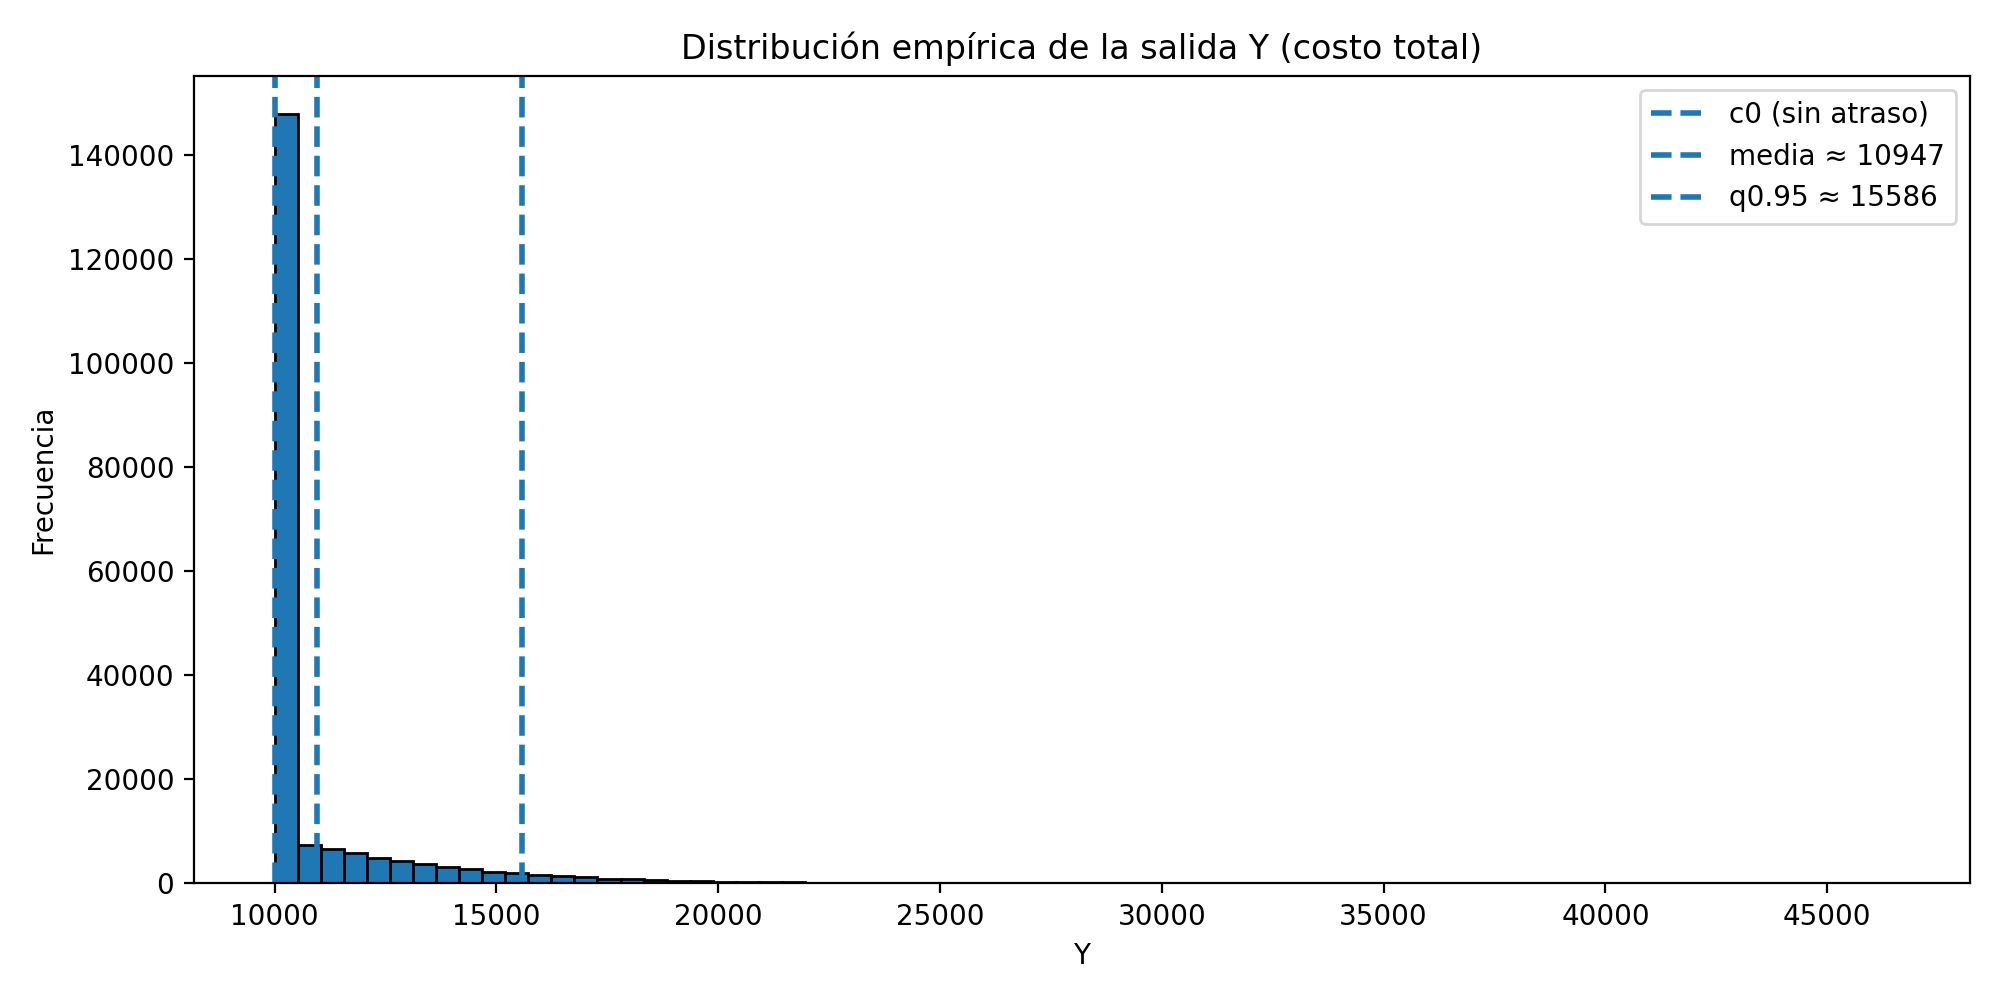
\includegraphics[width=0.95\textwidth]{fig_ex2_histY.png}

\begin{alertblock}{Mensaje conceptual}
En Monte Carlo, el resultado no es solo $\widehat{\mathbb E[Y]}$; también es una aproximación a la \textbf{distribución inducida} de $Y=g(\xi)$
(y por tanto a su \textbf{riesgo}).
\end{alertblock}
\end{frame}


\begin{frame}{Distribución de salida: CDF empírica y cuantiles (VaR como cuantil)}
\centering
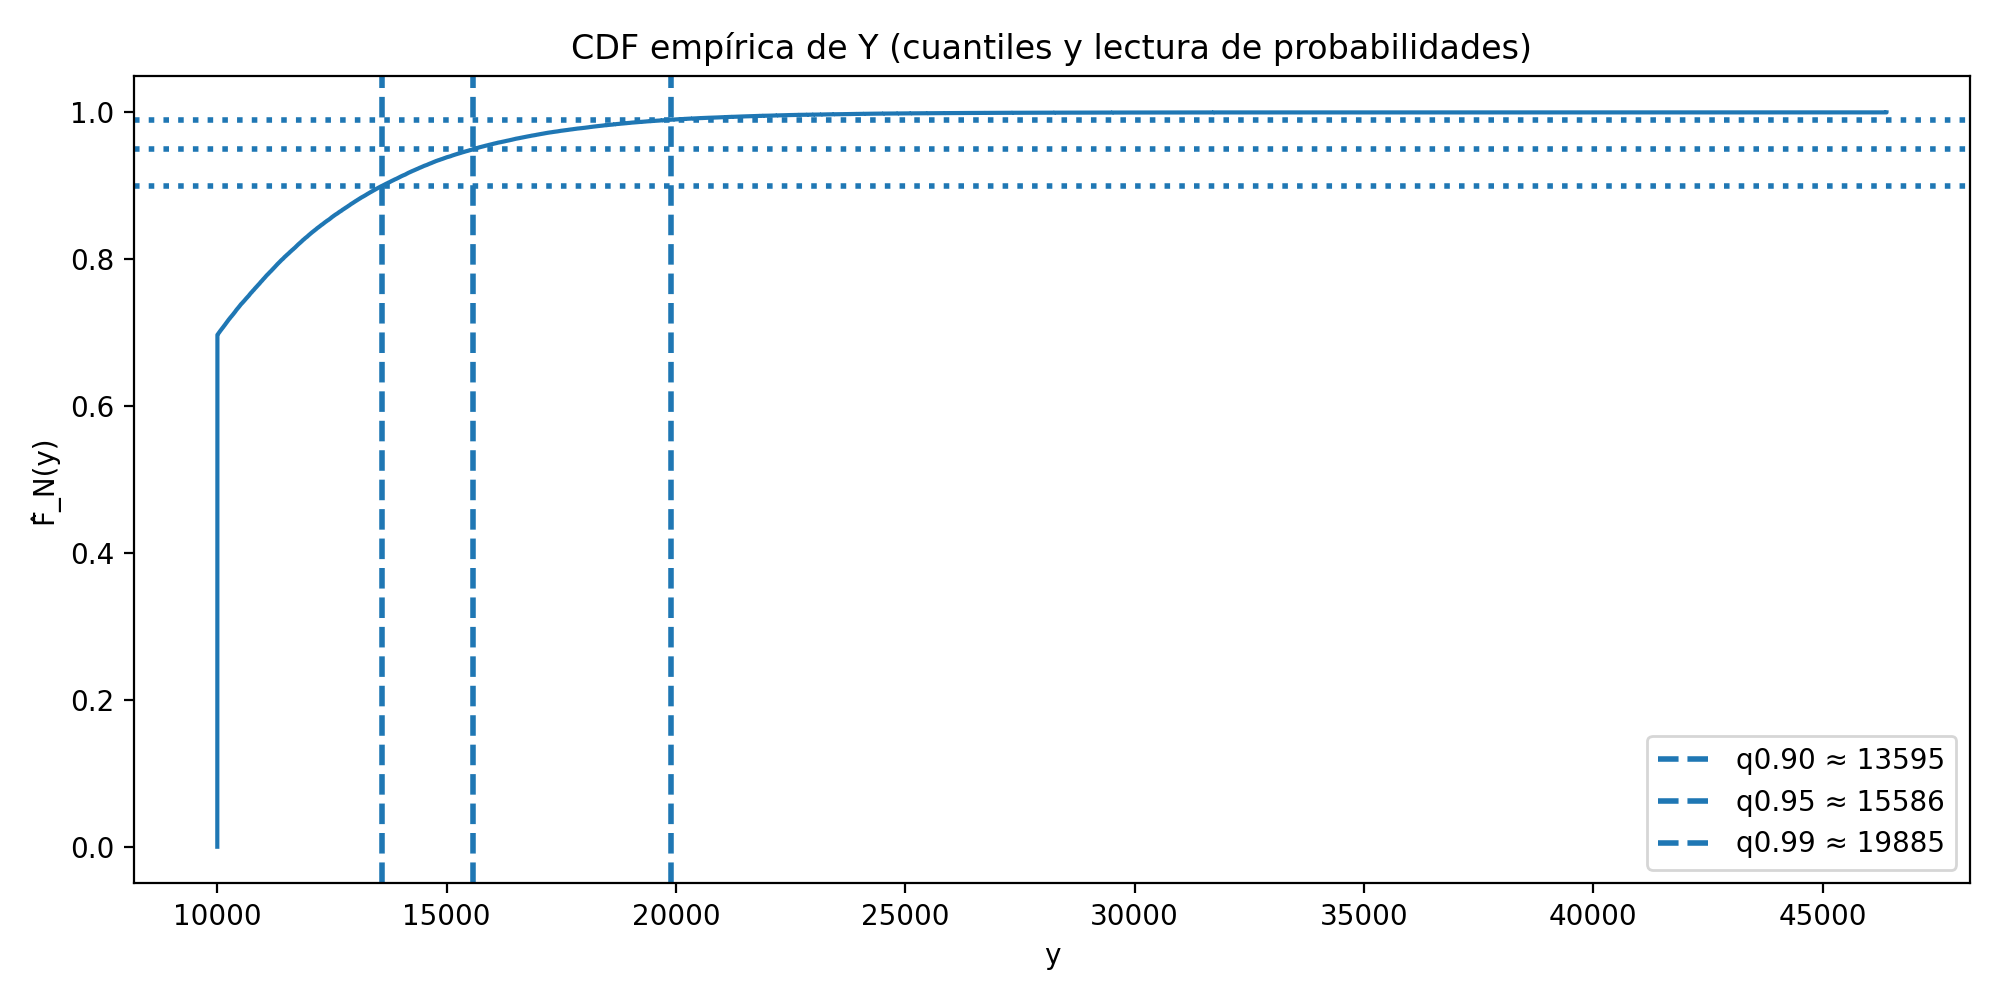
\includegraphics[width=0.95\textwidth]{fig_ex2_ecdfY.png}

\begin{block}{Interpretación}
La CDF empírica $\widehat F_N(y)$ permite leer directamente:
\[
q_{0.90}(Y),\ q_{0.95}(Y),\ \mathbb P(Y>\tau)=1-\widehat F_N(\tau).
\]
En particular, $q_{0.95}(Y)$ es el \textbf{percentil 95} (en finanzas se le llama VaR$_{0.95}$).
\end{block}
\end{frame}


\begin{frame}{Medidas derivadas de la distribución de salida}
\textbf{Parámetros usados en el ejemplo (días y costo):}
\[
d=6,\quad c_0=10000,\quad c_d=2000,
\qquad
L\sim \text{Lognormal}(\cdot,\sigma_{\log}=0.3),
\quad
S\sim \text{Gamma}(k=3,\theta=1).
\]

\medskip
\begin{block}{Estimaciones Monte Carlo típicas (p.ej.\ $N=2\cdot 10^5$, semilla fija)}
\begin{itemize}
  \item \textbf{Media:} $\widehat{\mu}=\widehat{\mathbb E[Y]}\approx 10947$.
  \item \textbf{Desv.\ estándar:} $\widehat{\sigma}_Y\approx 2138$.
  \item \textbf{Probabilidad de atraso:} $\widehat{\mathbb P}(T>d)\approx 0.303$.
  \item \textbf{Cuantiles:} $\widehat q_{0.90}(Y)\approx 13595$, \ $\widehat q_{0.95}(Y)\approx 15586$, \ $\widehat q_{0.99}(Y)\approx 19885$.
  \item \textbf{Medida de cola (CVaR$_{0.95}$):} $\widehat{\mathbb E[Y\mid Y\ge q_{0.95}]}\approx 18280$.
\end{itemize}
\end{block}

Media = costo esperado. Cuantiles/CVaR = \textbf{compromisos de servicio y riesgo} (``días malos típicos'' y ``cola extrema'').

\end{frame}


%================================================ % SLIDE 6: ERROR vs N (LLN + 1/sqrt(N)) %================================================ 

\begin{frame}{Error vs.\ $N$: por qué $1/\sqrt{N}$ aparece siempre}

\begin{block}{Ley de los grandes números (consistencia)} Si $Y_1,\dots,Y_N$ son i.i.d. y $\mathbb E[|Y|]<\infty$, entonces \[ \widehat\mu_N \longrightarrow \mu \quad \text{cuando } N\to\infty. \] Esto garantiza convergencia, pero no dice \emph{qué tan rápido}. 

\end{block}

\begin{block}{Tamaño típico del error (intuición)} La variabilidad de $\widehat\mu_N$ se reduce como \[ \mathrm{Var}(\widehat\mu_N)=\frac{\mathrm{Var}(Y)}{N} \qquad \Rightarrow \qquad \mathrm{SE}(\widehat\mu_N)=\frac{\sigma_Y}{\sqrt{N}}. \] 
\end{block} 

\begin{alertblock}{Regla práctica} Para mejorar precisión por un factor 2, necesitas aproximadamente 4 veces más réplicas. \end{alertblock} 
\end{frame}



\begin{frame}{Convergencia vs $n$: no solo la media (media, probabilidad y cuantil)}
\centering
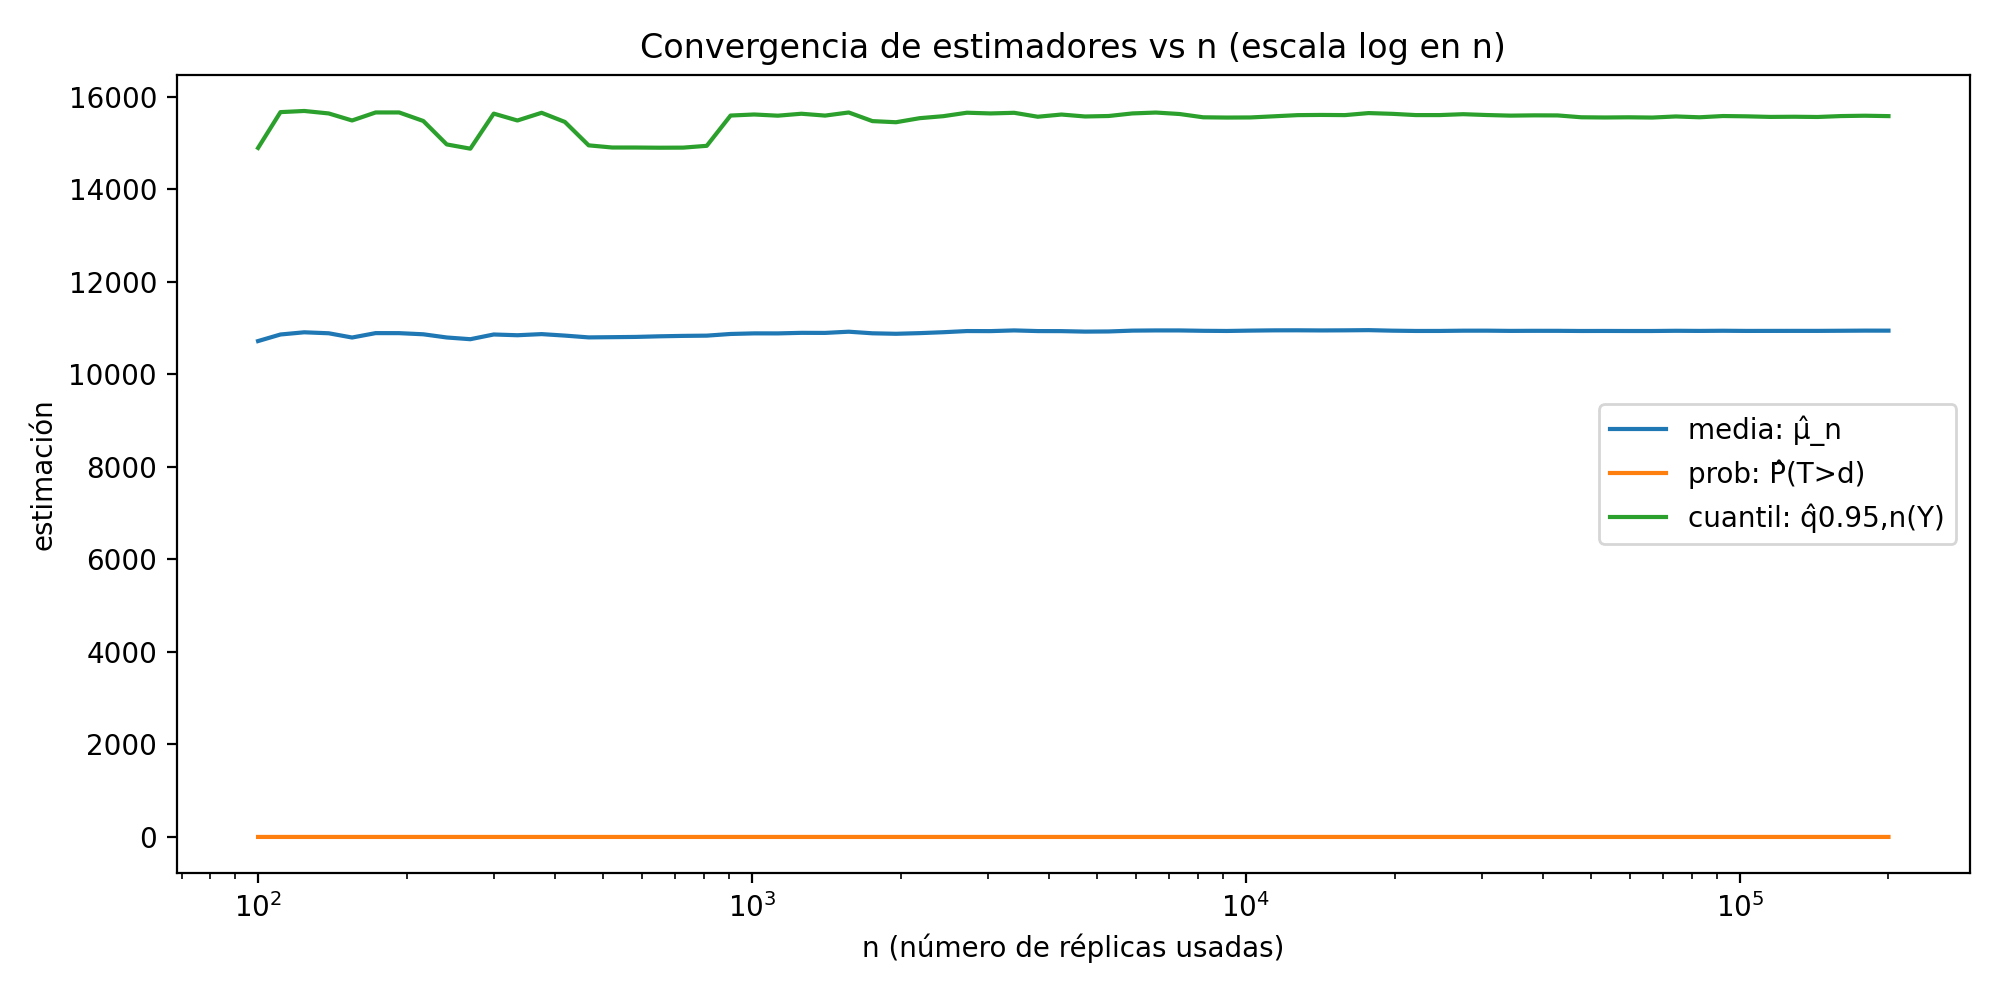
\includegraphics[width=0.95\textwidth]{fig_ex2_convergence.png}

\end{frame}

\begin{frame}{Convergencia vs.\ $n$ (cuatro estimadores, misma simulación)}
\centering
\begin{minipage}{0.49\linewidth}
  \centering
  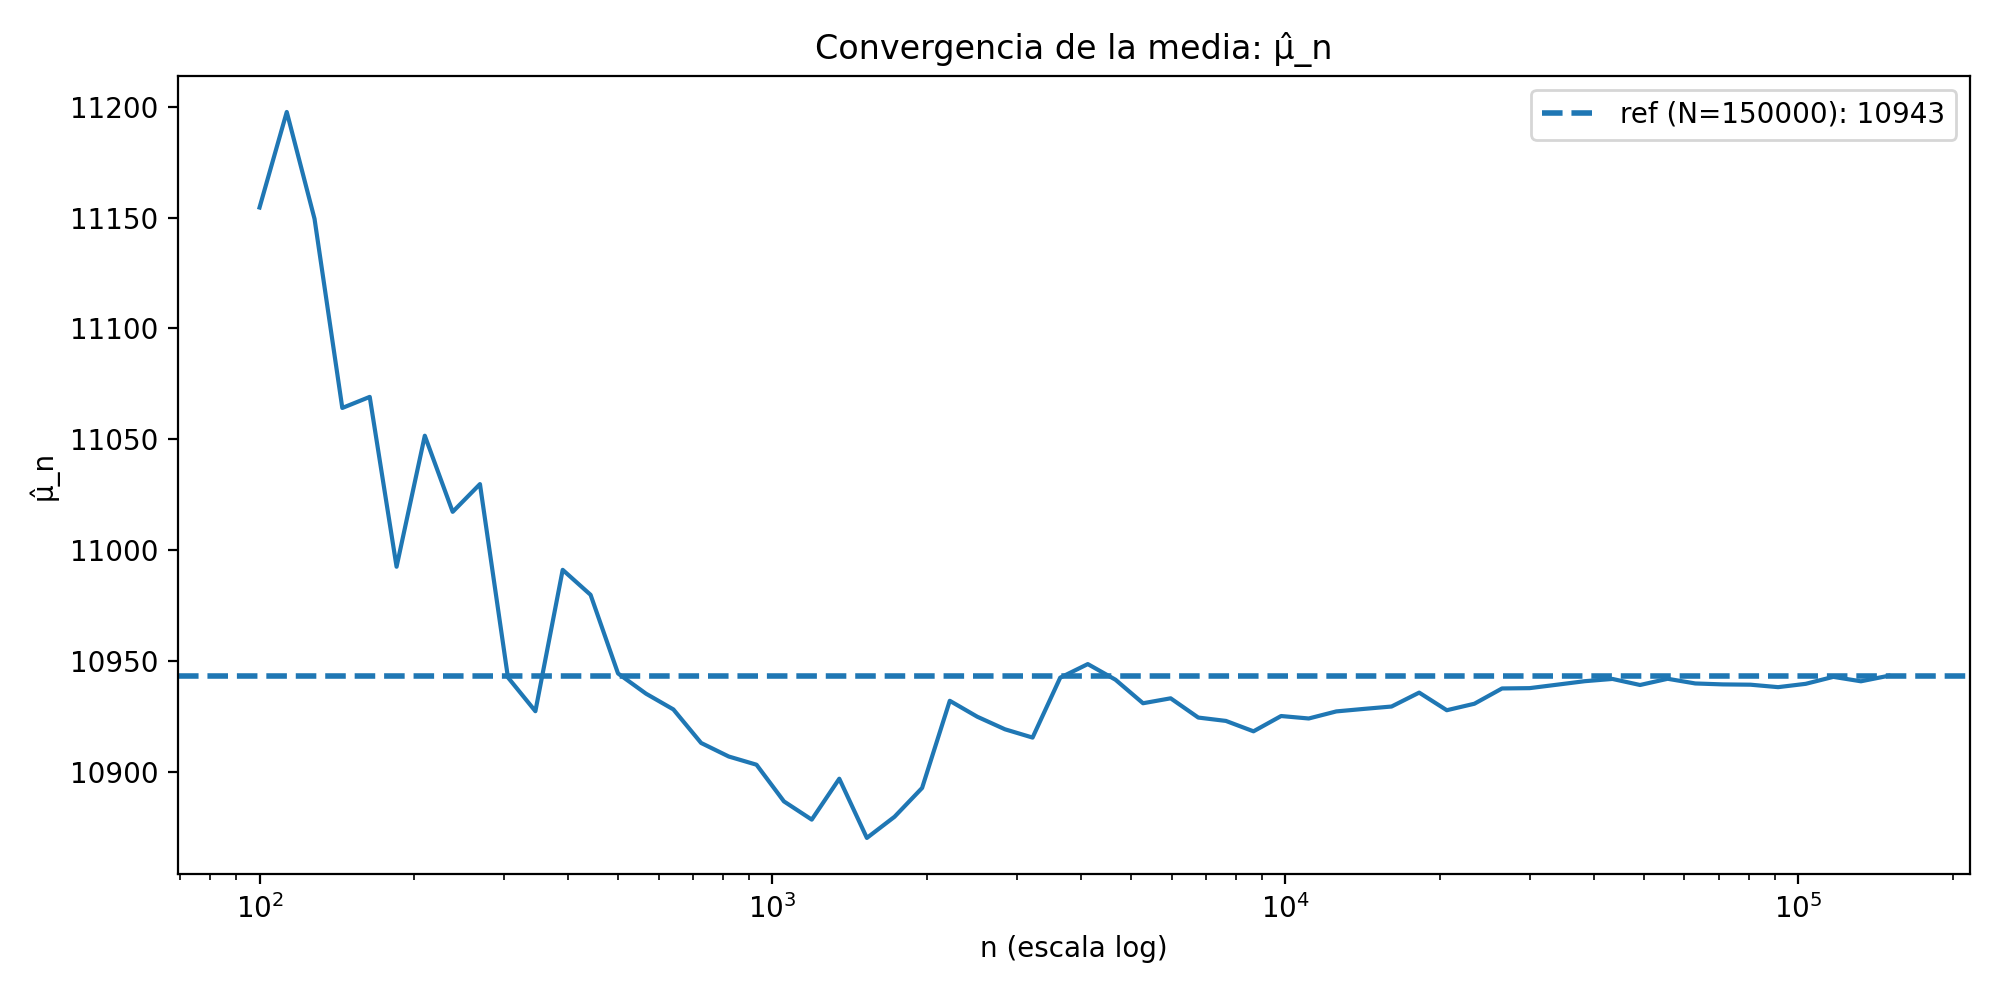
\includegraphics[width=\linewidth]{fig_ex2_conv_mean.png}\\[-0.2em]

\end{minipage}\hfill
\begin{minipage}{0.49\linewidth}
  \centering
  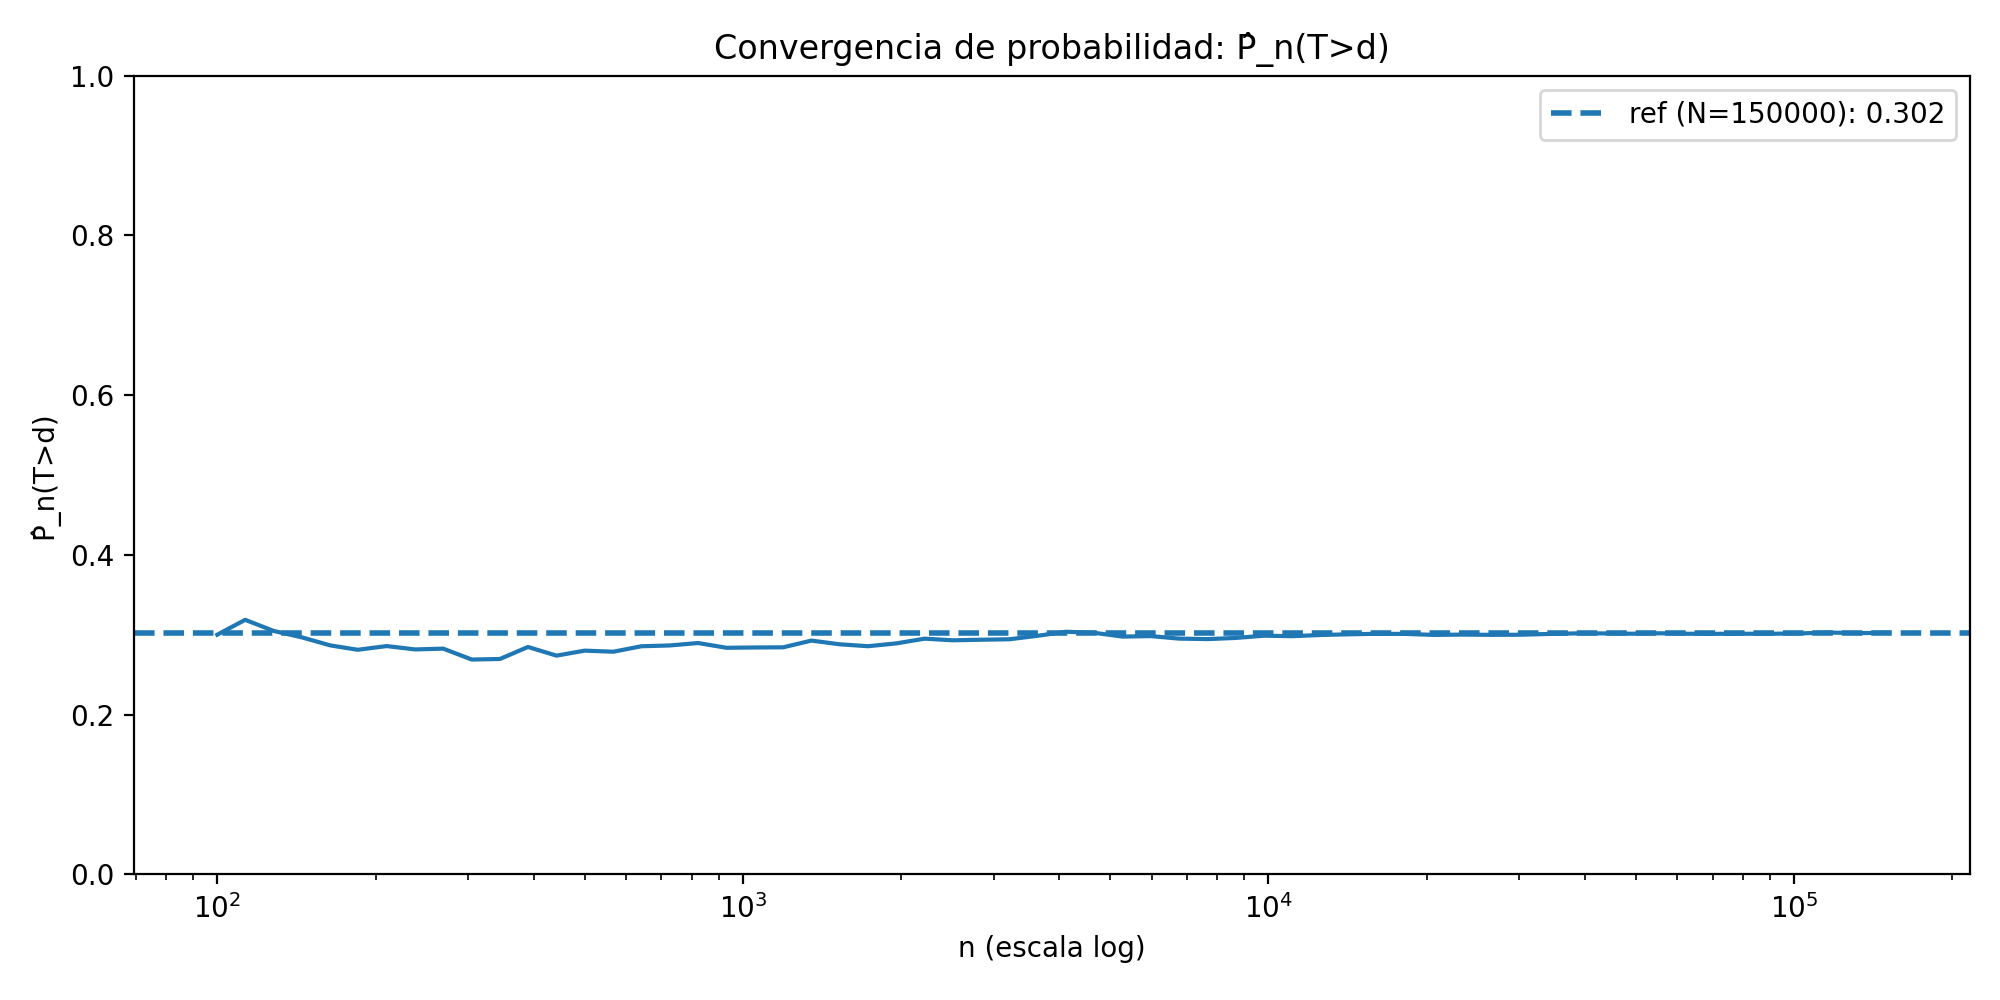
\includegraphics[width=\linewidth]{fig_ex2_conv_prob.png}\\[-0.2em]

\end{minipage}


\begin{minipage}{0.49\linewidth}
  \centering
  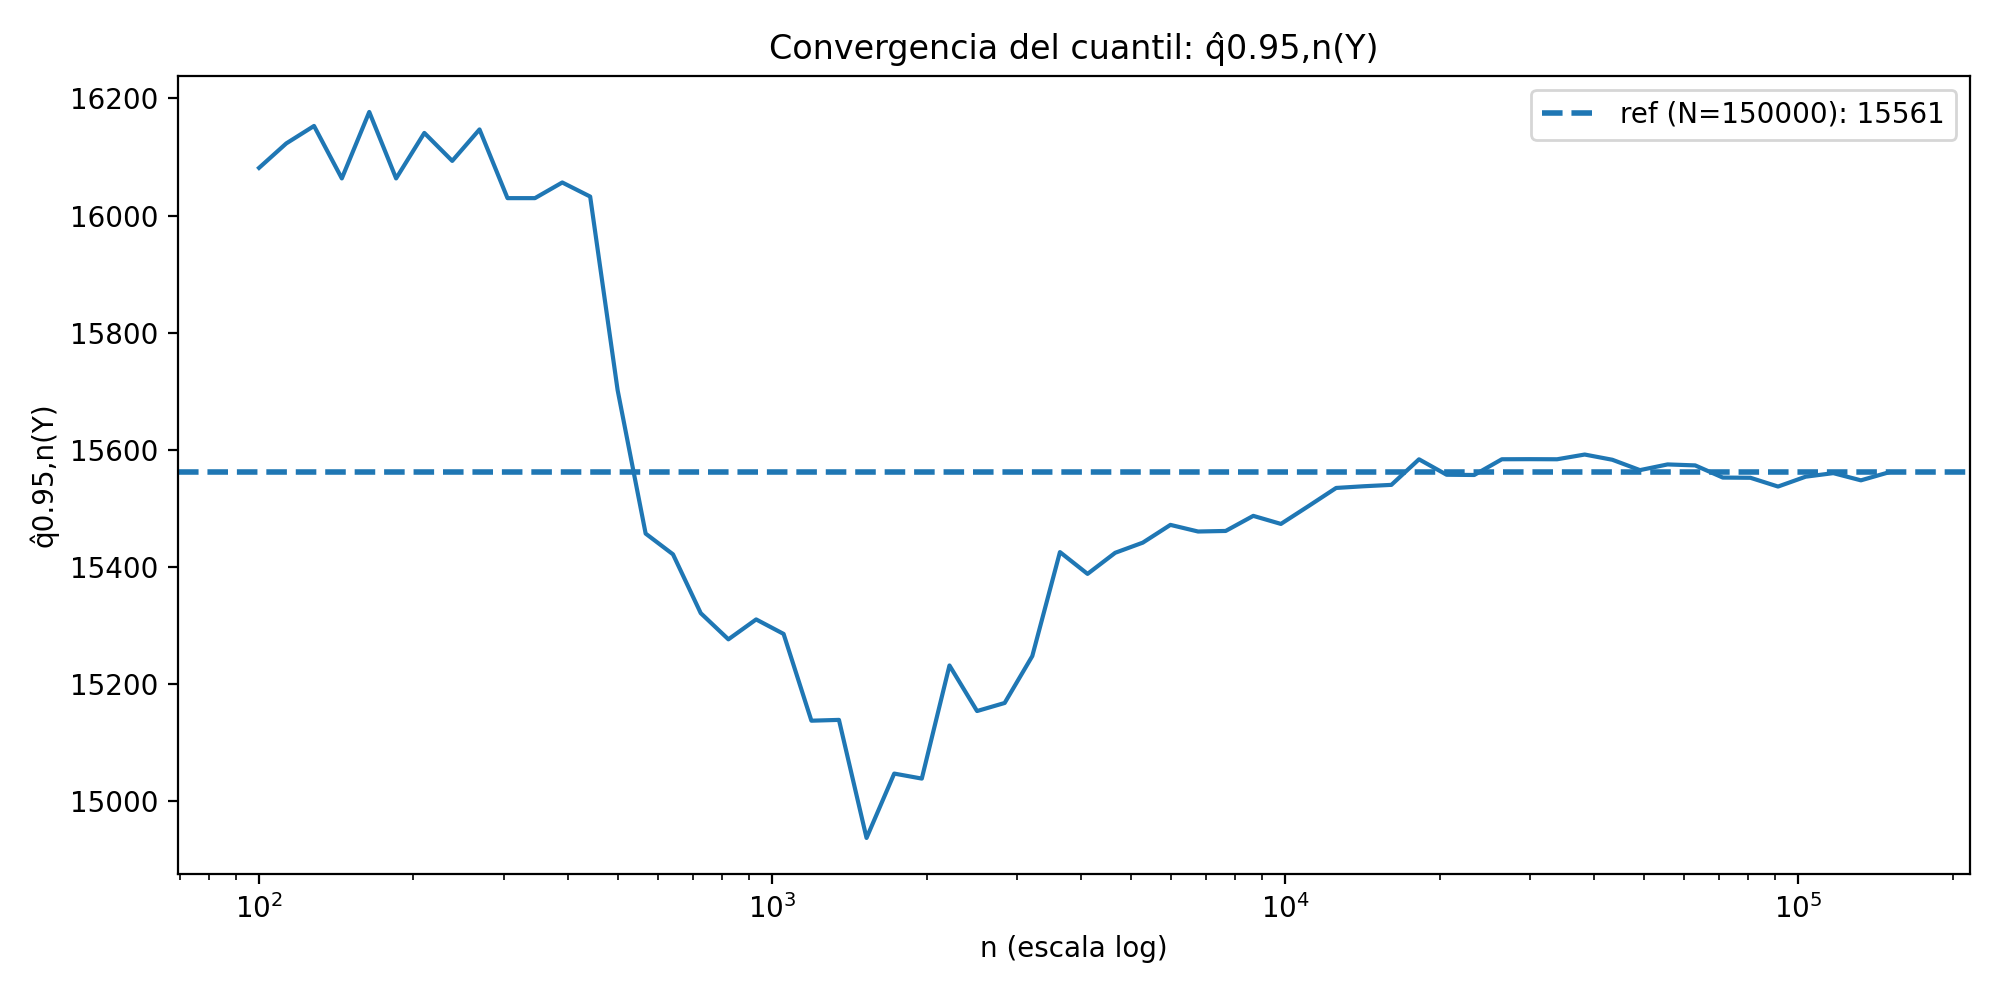
\includegraphics[width=\linewidth]{fig_ex2_conv_q95.png}\\[-0.2em]

\end{minipage}\hfill
\begin{minipage}{0.49\linewidth}
  \centering
  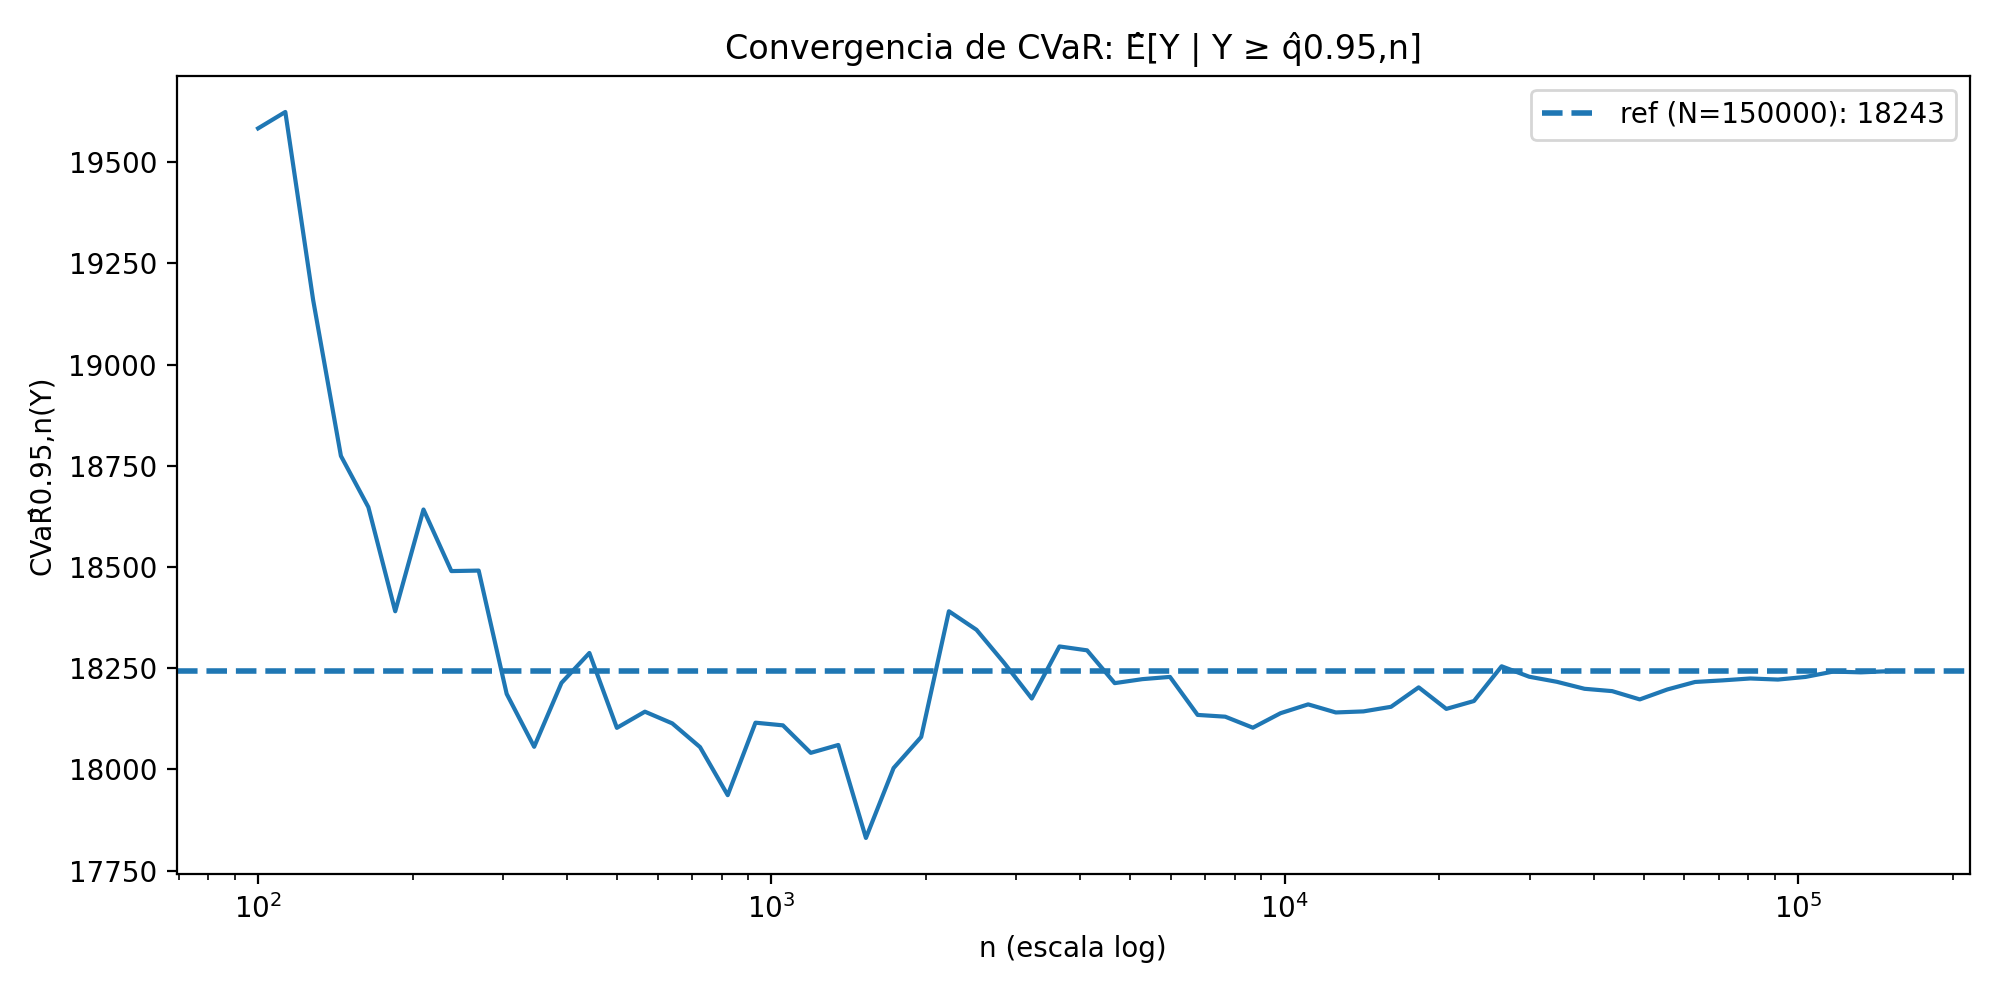
\includegraphics[width=\linewidth]{fig_ex2_conv_cvar95.png}\\[-0.2em]

\end{minipage}

\end{frame}


\begin{frame}{Dos objetos aleatorios distintos: salida $Y$ vs.\ estimador $\widehat\theta_N$}
\small
\begin{columns}[T]
\column{0.52\textwidth}
\begin{block}{1) Distribución de salida (incertidumbre del sistema)}
\[
Y=g(\xi)
\quad\Rightarrow\quad
F_Y(y)=\mathbb P(Y\le y).
\]
Aquí \textbf{$Y$ es el resultado} de \emph{un día / un escenario} (una corrida).

\medskip
\textbf{¿Cómo se mira?} Con histograma o CDF empírica $\widehat F_N$ construida con $\{Y_i\}$.

\medskip
\textbf{¿Qué deriva de $F_Y$?}
\[
\mathbb E[Y],\qquad \mathbb P(Y>\tau),\qquad q_\alpha(Y),\qquad \mathrm{CVaR}_\alpha(Y).
\]
\end{block}

\column{0.48\textwidth}
\begin{block}{2) Distribución del estimador (error Monte Carlo)}
\[
\widehat\theta_N=\widehat\theta_N(Y_1,\dots,Y_N)
\ \ \text{también es aleatorio.}
\]
Porque cambia si vuelves a simular con \emph{otra} muestra i.i.d.

\medskip
\textbf{Idea clave:} si repites el experimento completo muchas veces
(\textbf{muchos “Monte Carlo de Monte Carlo”}),
obtienes una \textbf{distribución de muestreo} de $\widehat\theta_N$.

\medskip
\textbf{Eso justifica} barras de error, error estándar e intervalos de confianza.
\end{block}
\end{columns}

\begin{alertblock}{}
\textbf{La nube $\{Y_i\}$ describe el sistema.} \quad
\textbf{La variabilidad de $\widehat\theta_N$ describe tu incertidumbre por usar $N$ finito.}
\end{alertblock}
\end{frame}



\begin{frame}{Dos objetos aleatorios distintos: salida $Y$ vs estimador $\widehat\theta_N$}
\begin{columns}[T]
\column{0.45\textwidth}

\medskip
\centering
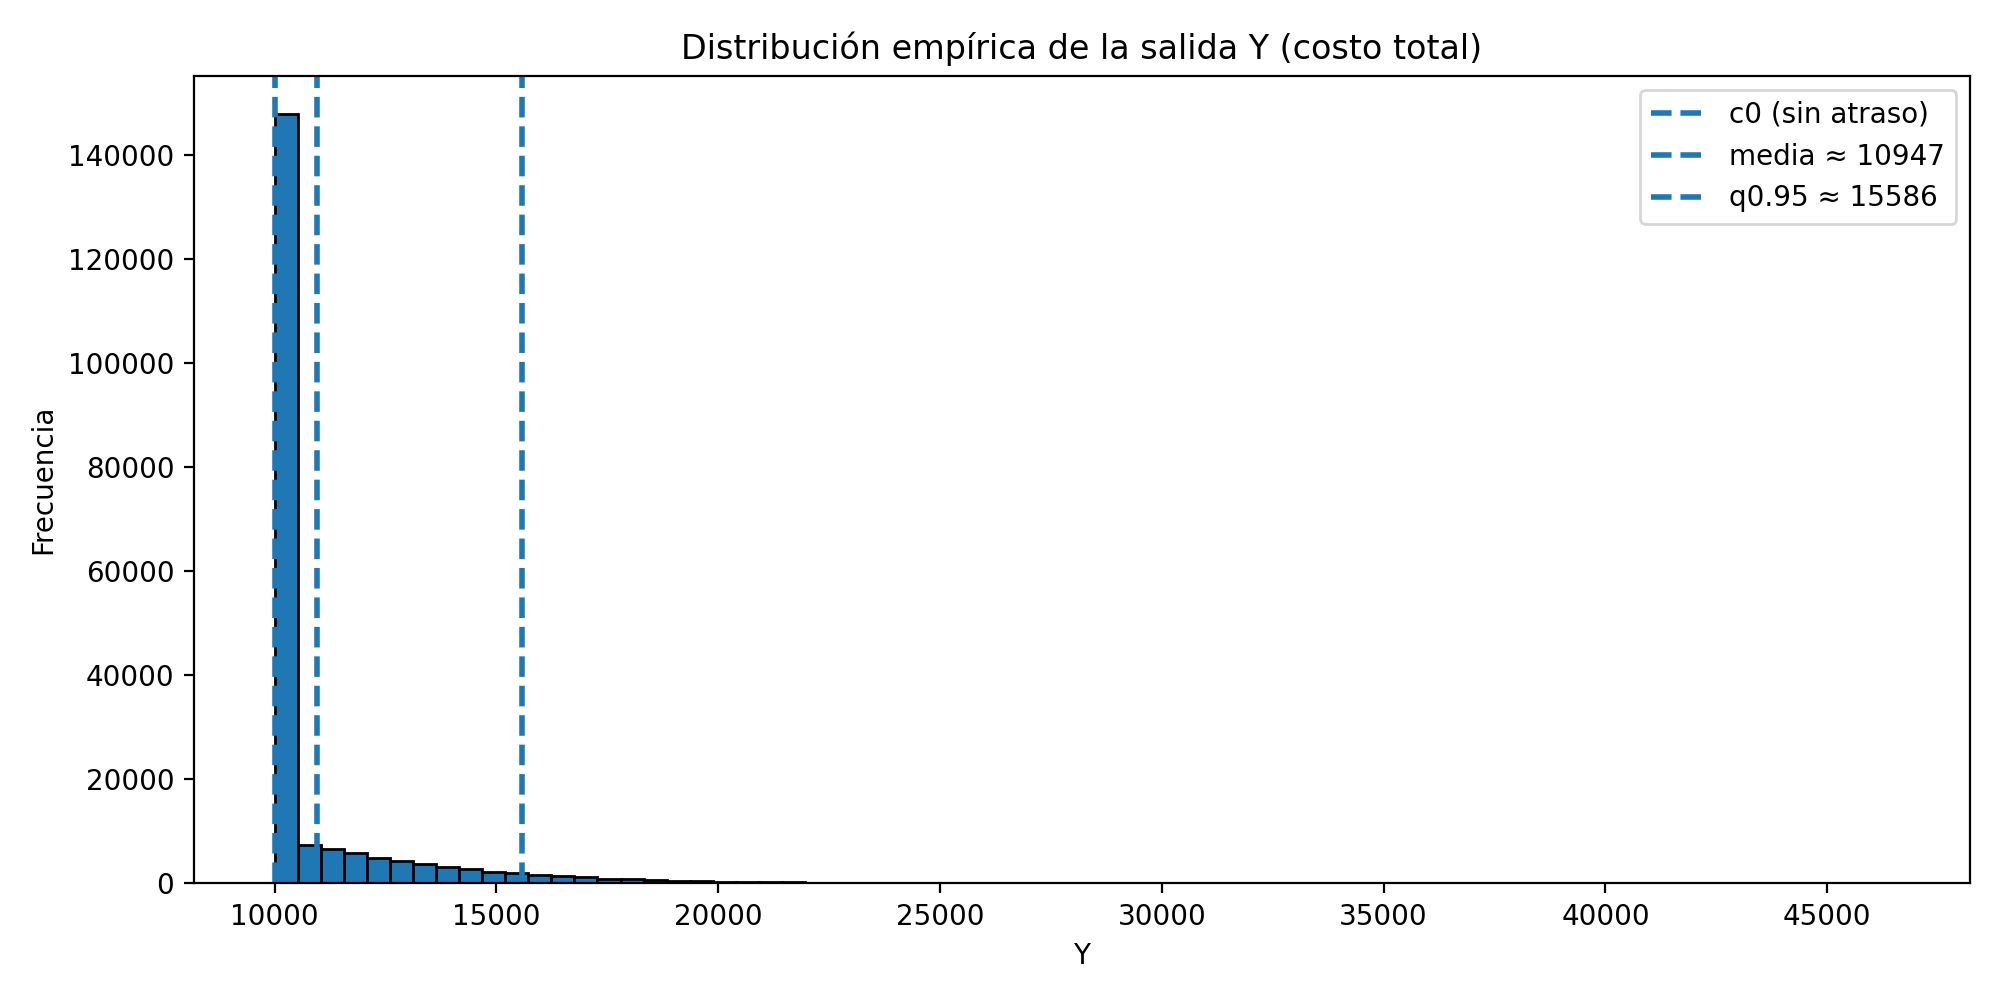
\includegraphics[width=0.95\textwidth]{fig_ex2_histY.png}

\column{0.45\textwidth}

\medskip
\centering
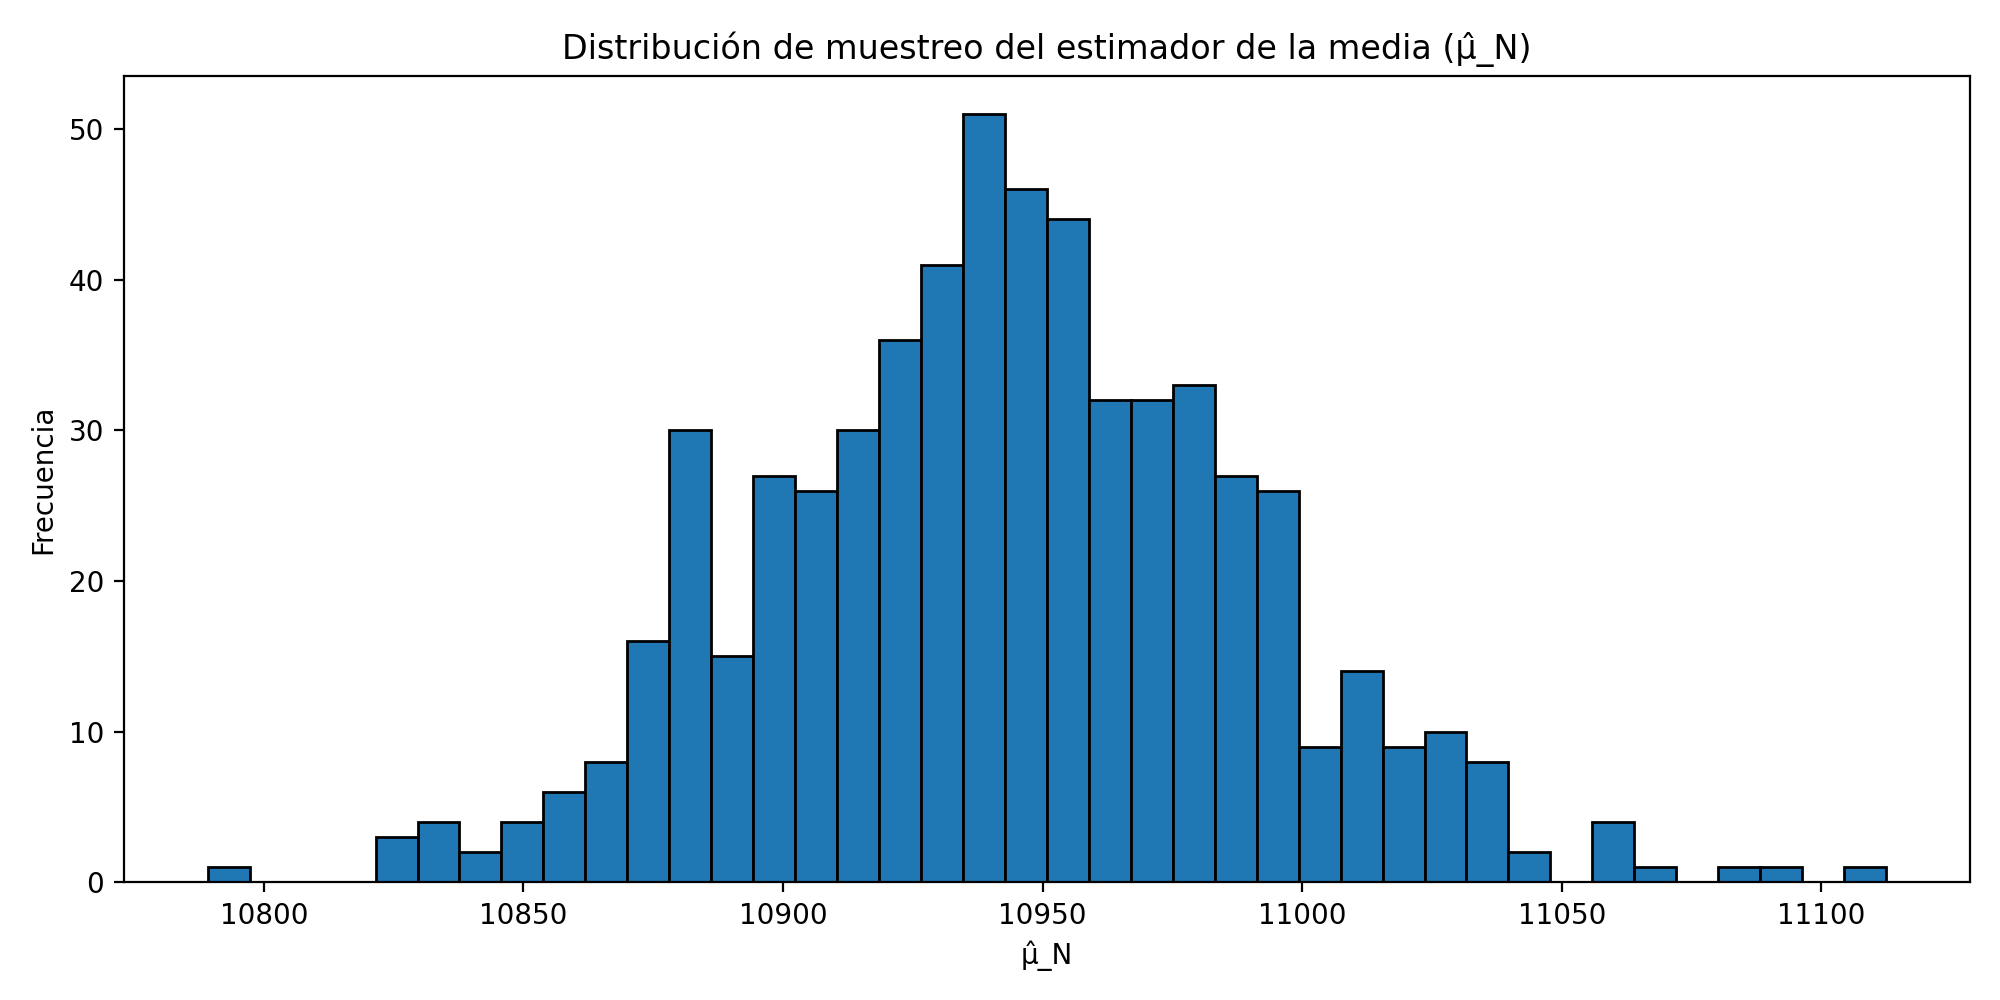
\includegraphics[width=0.95\textwidth]{fig_ex2_sampling_mean.png}
\end{columns}

\end{frame}


\begin{frame}{Distribución del estimador: ejemplo con un cuantil}
\centering
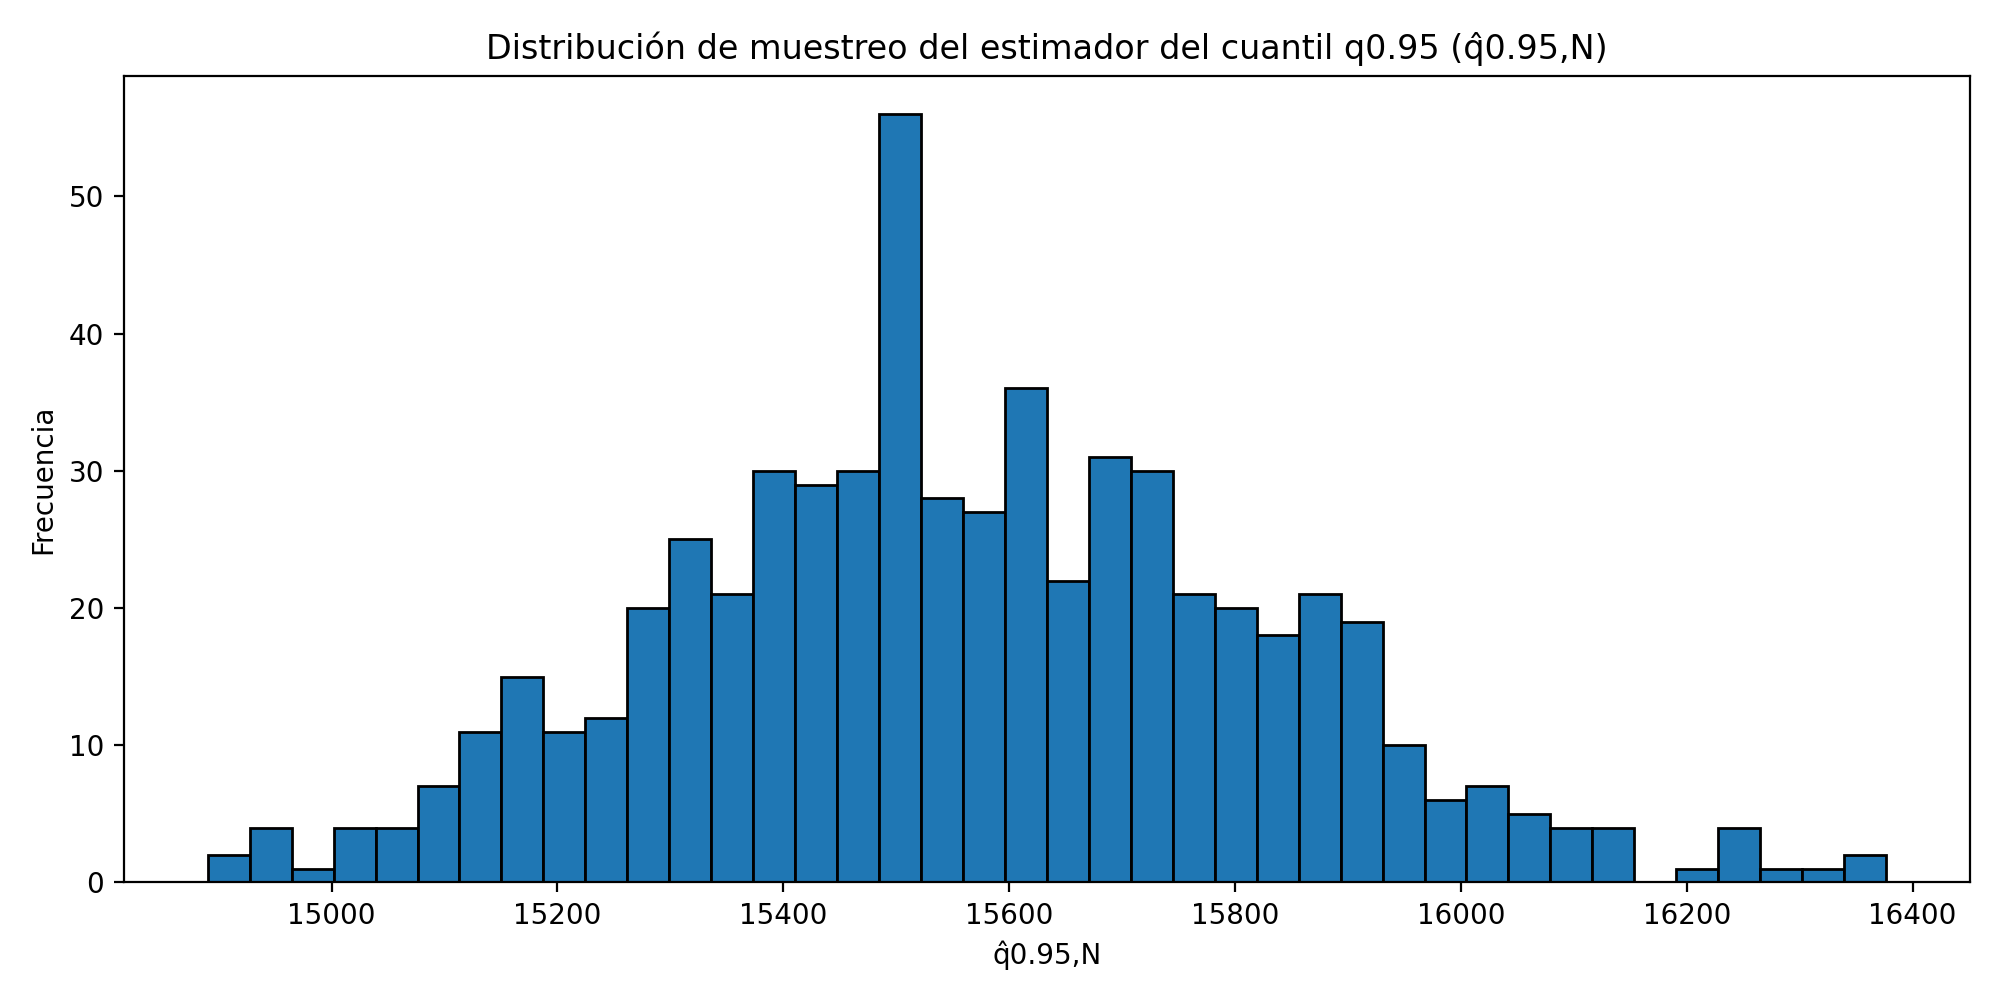
\includegraphics[width=0.95\textwidth]{fig_ex2_sampling_quantile.png}

\begin{alertblock}{Mensaje práctico}
El cuantil (p.ej.\ $q_{0.95}$) es un funcional de cola: su variabilidad muestral puede ser alta si $N$ no es grande.
Por eso \textbf{percentiles altos} necesitan \textbf{muchas más réplicas} que la media.
\end{alertblock}
\end{frame}

\begin{frame}{Distribución del estimador: media vs probabilidad (repetir el MC completo)}
\begin{columns}
\column{0.5\textwidth}
\centering
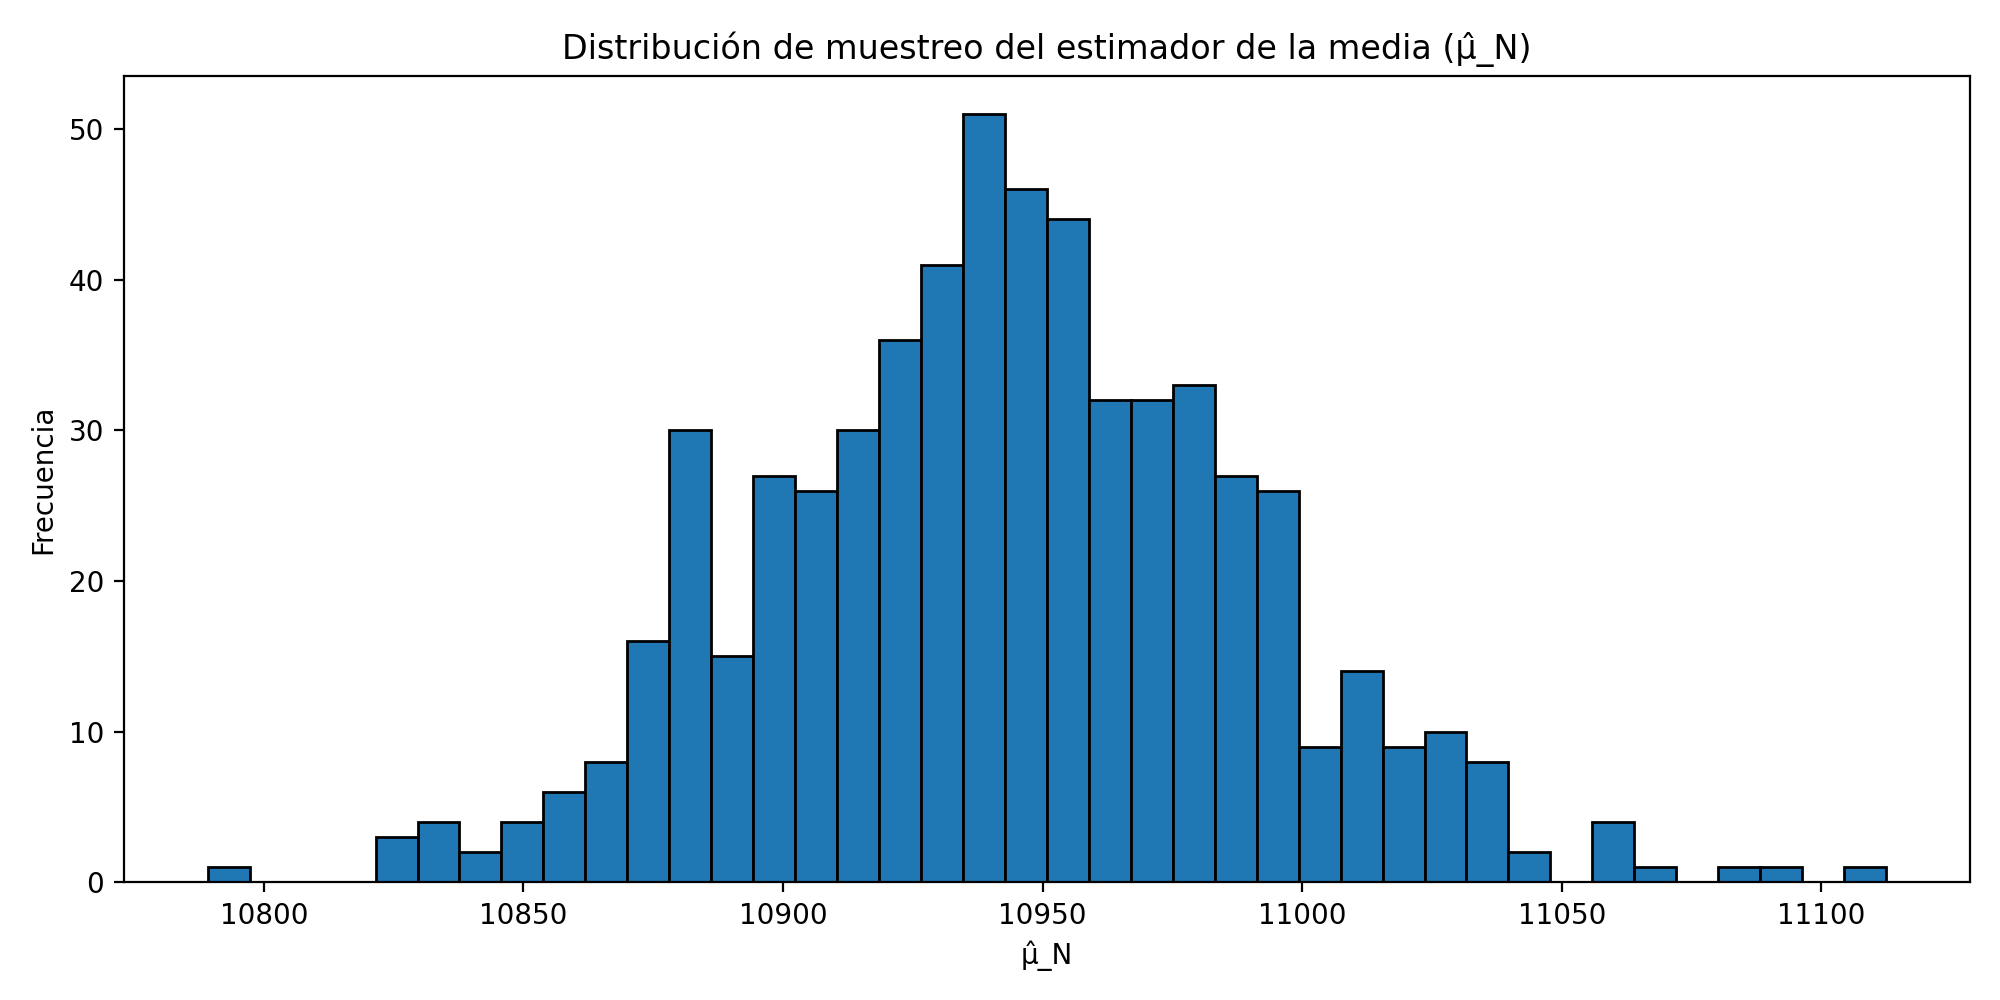
\includegraphics[width=\textwidth]{fig_ex2_sampling_mean.png}

\column{0.5\textwidth}
\centering
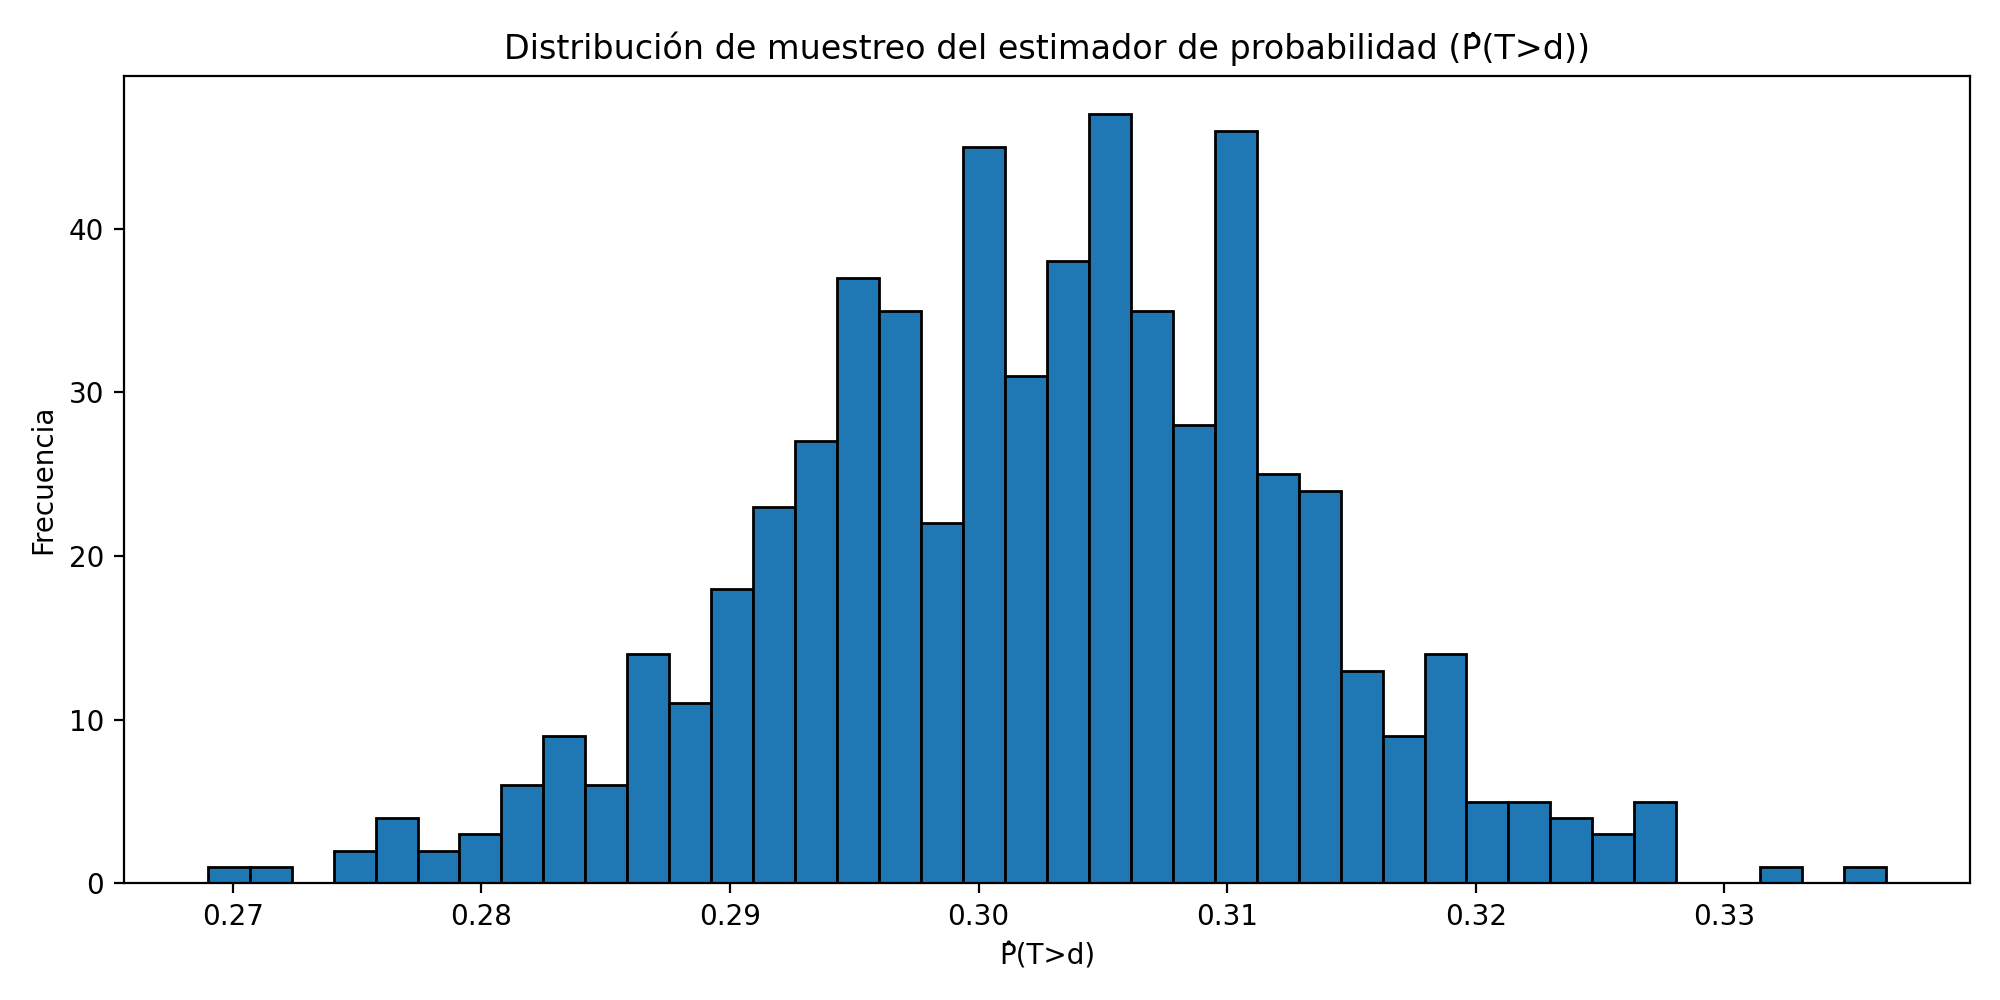
\includegraphics[width=\textwidth]{fig_ex2_sampling_prob.png}
\end{columns}
\end{frame}



%================================================
% SLIDE 8: SEMILLAS Y REPRODUCIBILIDAD
%================================================
\begin{frame}{Semillas y reproducibilidad: lo computacional también es estadística}
\begin{block}{Qué controla una semilla}
El generador pseudoaleatorio produce una secuencia determinista larga. Fijar \texttt{seed} significa:
\[
\text{misma semilla} \Rightarrow \text{misma secuencia} \Rightarrow \text{mismos } Y_1,\dots,Y_N.
\]
Esto es crucial para \textbf{reproducibilidad} y depuración.
\end{block}

\begin{block}{Qué NO garantiza una semilla}
Una semilla no ``hace más verdadero'' el resultado; solo lo hace replicable.
La validez estadística depende de (i) independencia aproximada, (ii) modelo probabilístico, (iii) tamaño muestral.
\end{block}

\begin{alertblock}{Buena práctica mínima}
Reportar: semilla, $N$, y definición exacta de $Y=g(\xi)$ (para que el experimento sea replicable).
\end{alertblock}
\end{frame}

%================================================
% SLIDE 9: GENERACIÓN DE VA (inversa / transformaciones / numpy)
%================================================
\begin{frame}{Generación de variables aleatorias: 3 rutas complementarias}
\begin{block}{Ruta A: generadores directos (\texttt{numpy.random})}
Cuando existe un generador implementado, se usa directamente: Normal, Poisson, Exponencial, Uniforme, etc.
\end{block}

\begin{block}{Ruta B: transformaciones (construir desde algo simple)}
Si $U\sim \mathrm{Unif}(0,1)$:
\[
X=a+(b-a)U \sim \mathrm{Unif}(a,b).
\]
Si $X_1,\dots,X_k$ son Exponenciales i.i.d., su suma es Gamma/Erlang (modelo de ``k etapas'').
\end{block}

\begin{block}{Ruta C: método inverso (principio general)}
Si $U\sim\mathrm{Unif}(0,1)$ y $F$ es una cdf, entonces $X=F^{-1}(U)$ tiene distribución $F$.
\emph{Ejemplo:} si $X\sim\mathrm{Exp}(\lambda)$, entonces $F^{-1}(u)=-\frac{1}{\lambda}\ln(1-u)$.
\end{block}
\end{frame}

%================================================
% SLIDE 10: EJEMPLO 1 (BERNOULLI) + IC (con interpretación)
%================================================
\begin{frame}[fragile]{Ejemplo 1 (simple): Bernoulli y el IC que ``se ve''}
\textbf{Situación:} un componente pasa una prueba con probabilidad desconocida $p$.
Definimos $X=1$ si pasa y $0$ si falla. Entonces $X\sim \mathrm{Bernoulli}(p)$ y $\mu=\mathbb E[X]=p$.


\begin{block}{Interpretación}
El IC se estrecha como $1/\sqrt{N}$: si quieres la mitad del ancho, necesitas $\approx 4N$.
\end{block}
\end{frame}

%================================================
% SLIDE 11: EJEMPLO 2 (ING. INDUSTRIAL): INVENTARIO / FALTANTE
%================================================
\begin{frame}[fragile]{Ejemplo 2 (Ing.\ Industrial): faltantes en inventario (media, prob, cuantil)}
\textbf{Situación:} se ordena una cantidad fija $Q$ para mañana. La demanda $D$ es incierta.
El costo por faltante es $c_s$ por unidad:
\[
Y=c_s(D-Q)_+.
\]
Aquí $Y$ es la \textbf{salida} y su distribución suele ser \textbf{muy asimétrica} (muchos ceros, cola derecha).


\begin{alertblock}{Lectura}
La media resume costo esperado; $\mathbb P(Y>\tau)$ captura riesgo operacional; $q_{0.90}$ responde ``¿qué tan malo es un día malo típico?''.
\end{alertblock}
\end{frame}

%================================================
% SLIDE 12: DIAGNÓSTICOS (histograma + media corrida)
%================================================
\begin{frame}[fragile]{Diagnóstico básico: histograma y convergencia de la media}
Monte Carlo no solo entrega números: también exige \textbf{diagnósticos} mínimos.

\begin{block}{Dos diagnósticos que siempre deberían existir}
(1) Histograma (forma/colas) $\Rightarrow$ te recuerda que $Y$ tiene distribución. \\
(2) Media corrida $\widehat\mu_n$ vs.\ $n$ $\Rightarrow$ te muestra estabilidad del estimador.
\end{block}

\end{frame}


%================================================
% SLIDE 14: CIERRE CON REPASO CONCEPTUAL + EJERCICIOS
%================================================
%================================================
% EJERCICIOS (bloque nuevo): conceptos + Python
%================================================

%------------------------------------------------
% EJERCICIO 1: identificar objetos (xi, g, Y, theta, estimador)
%------------------------------------------------
%------------------------------------------------
% EJERCICIO 1 (reemplazo): modelar situaciones + formular preguntas + elegir métricas
%------------------------------------------------
\begin{frame}{Ejercicio 1: modelar la incertidumbre y elegir \emph{qué} preguntar}
\small
En Monte Carlo, el paso más difícil (y más importante) suele ser \textbf{antes} de simular:
\textbf{definir el modelo} y \textbf{definir qué pregunta cuantitativa} se quiere responder.

\begin{block}{Tres situaciones}
Para \textbf{una} de las siguientes situaciones (escoja la que prefiera):
\begin{enumerate}
  \item \textbf{Turnos en un servicio:} llegan clientes y se forman filas; le preocupa el nivel de espera.
  \item \textbf{Transporte urbano:} el tiempo de viaje cambia por tráfico e incidentes; hay hora de llegada compromiso.
  \item \textbf{Mantenimiento industrial:} una máquina puede fallar; hay tiempo de reparación y costo por paro.
\end{enumerate}
\end{block}

\begin{block}{Tarea: proponer un modelo (pensar, no copiar)}
Defina, en palabras y en símbolos:
\[
\xi\ \text{(fuentes de incertidumbre)}\quad\Rightarrow\quad Y=g(\xi)\ \text{(salida de interés)}.
\]
\textbf{Regla:} use al menos \textbf{dos} componentes aleatorios en $\xi$ (p.ej.\ llegada + servicio; tráfico + incidentes; falla + reparación).
No necesita poner distribuciones exactas todavía: basta con justificar \emph{qué} es aleatorio y por qué.
\end{block}

\end{frame}



%------------------------------------------------
% EJERCICIO 2: LLN vs CLT vs IC (conceptual + operativo)
%------------------------------------------------
\begin{frame}{Ejercicio 2: LLN vs CLT vs IC (¿qué te da cada uno?)}
\small
Después de simular obtienes números $Y_1,\dots,Y_N$.

\begin{block}{Parte A (conceptual)}
Marque con \textbf{V/F} y justifique en una línea:
\begin{enumerate}
\item ``La LLN me dice el ancho del intervalo de confianza.'' \hfill (\ \ )
\item ``El CLT justifica aproximar la distribución de $\widehat\mu_N$ por una Normal.'' \hfill (\ \ )
\item ``Un IC para $\mu$ también es un IC para un día típico $Y$.'' \hfill (\ \ )
\end{enumerate}
\end{block}

\begin{block}{Parte B (operativa)}
Si quiere \textbf{mitad} del ancho del IC de $\mu$, ¿cuántas réplicas necesita en términos de $N$?
\[
\text{ancho} \propto \frac{1}{\sqrt{N}} \qquad \Rightarrow \qquad N_{\text{nuevo}}=\ ? 
\]
\end{block}
\end{frame}


%------------------------------------------------
% EJERCICIO 3: salida vs estimador (dos distribuciones)
%------------------------------------------------
\begin{frame}{Ejercicio 3: dos distribuciones distintas (y dos gráficas distintas)}
\small
En Monte Carlo conviven dos objetos aleatorios:

\begin{block}{1) Distribución de salida}
La muestra $\{Y_i\}$ aproxima $F_Y$ (histograma, CDF empírica, cuantiles, colas).
\end{block}

\begin{block}{2) Distribución del estimador}
El número $\widehat\mu_N$ cambia si repites el experimento completo $\Rightarrow$ tiene distribución de muestreo.
\end{block}

\begin{block}{Tarea}
\begin{enumerate}
\item Escriba una frase: \textbf{¿qué pregunta contesta} el histograma de $Y$?
\item Escriba una frase: \textbf{¿qué pregunta contesta} el histograma de $\widehat\mu_N$?
\item En el ejemplo del atraso: ¿cuál de las dos distribuciones usaría para hablar de \textbf{riesgo} y por qué?
\end{enumerate}
\end{block}
\end{frame}


%------------------------------------------------
% EJERCICIO 4: primer MC en Python (rellenar huecos) - Bernoulli + IC
%------------------------------------------------
\begin{frame}[fragile]{Ejercicio 4: Bernoulli en Python (rellenar huecos + IC)}
\small
\textbf{Objetivo:} estimar $p=\mathbb E[X]$ con $X\sim \text{Bernoulli}(p)$ y reportar IC 95\%.


\begin{block}{Preguntas}
(i) ¿Qué cambia si $N$ pasa de 2000 a 8000? \quad
(ii) ¿Por qué aquí el IC se puede construir con CLT?
\end{block}
\end{frame}


%------------------------------------------------
% EJERCICIO 5: inventario (continuo) + 3 métricas (media, prob, cuantil)
%------------------------------------------------
\begin{frame}[fragile]{Ejercicio 5: inventario (continuo) + 3 métricas}
\small
\textbf{Modelo:} $D\sim \mathcal N(\mu,\sigma^2)$ truncada a no-negativa.
\[
Y=c_s(D-Q)_+.
\]
Use: $\mu=100,\ \sigma=30,\ Q=100,\ c_s=10,\ N=30000$.


\begin{block}{Tarea}
Cambie SOLO una cosa a la vez:
(i) $\sigma=50$ \quad (ii) $Q=120$ \quad (iii) $\tau=400$.
Explique en palabras qué cambia en (a), (b), (c).
\end{block}
\end{frame}


%------------------------------------------------
% EJERCICIO 6: gráficos mínimos (salida + convergencia) - práctica Python
%------------------------------------------------
\begin{frame}[fragile]{Ejercicio 6: diagnósticos mínimos (2 gráficos obligatorios)}
\small
\textbf{Objetivo:} producir \textbf{dos gráficos} para el ejercicio anterior: (1) histograma de $Y$, (2) media corrida $\widehat\mu_n$.


\begin{block}{Preguntas}
(i) ¿Qué te dice el histograma que la media NO te dice? \quad
(ii) ¿Cómo se ve la convergencia si duplicas $N$?
\end{block}
\end{frame}


%------------------------------------------------
% EJERCICIO 7: depuración guiada (muy útil para principiantes)
%------------------------------------------------
\begin{frame}[fragile]{Ejercicio 7: depuración (encuentre y corrija 4 errores)}
\small
Este código \textbf{pretende} estimar $\mathbb E[Y]$ para $Y=c_s(D-Q)_+$, pero tiene errores.


\begin{block}{Tarea}
Identifique y corrija \textbf{cuatro} errores. Luego corra y reporte $E[Y]$.
\end{block}
\end{frame}


%------------------------------------------------
% EJERCICIO 8: modelado (distribuciones para xi) con contexto (sin pistas excesivas)
%------------------------------------------------
\begin{frame}{Ejercicio 8: modelar $\xi$ (¿qué distribución usarías y por qué?)}
\small
En cada caso, proponga una distribución para la \textbf{entrada aleatoria} y justifique con \textbf{dos razones}
(soporte, forma, mecanismo, cola, discreto/continuo).

\begin{enumerate}
\item Caso A: tiempo entre llegadas a una ventanilla; hay pausas y ráfagas.
\item Caso B: duración total de una tarea con 3 etapas consecutivas.
\item Caso C: número de llamadas por hora en un call center.
\item Caso D: duración estimada por experto con (optimista, más probable, pesimista).
\end{enumerate}

\begin{alertblock}{Regla}
Primero describa el soporte y el mecanismo; \textbf{luego} proponga distribución.
\end{alertblock}
\end{frame}

\end{document}
